\documentclass[12pt]{article}
% my packages
\usepackage{fullpage}
\usepackage{graphicx}
\usepackage{amsmath}
\usepackage{amsthm}
\usepackage{amssymb}
\usepackage{mathtools}
\usepackage{verbatim}
\usepackage{color}
\usepackage{boxedminipage}
\usepackage{slashbox}
\usepackage{enumitem}
\usepackage[caption=false]{subfig}
\usepackage{url}
\usepackage{listings}
\usepackage{xcolor}
\usepackage{hyperref}

\definecolor{commentcolor}{rgb}{0,0.6,0}
\definecolor{keywordcolor}{rgb}{0,0,0.8}
\definecolor{numbercolor}{rgb}{0.5,0.5,0.5}
\definecolor{stringcolor}{rgb}{0.58,0,0.82}
\lstset{%
    language=Verilog,                        % closest to BSV
    backgroundcolor=\color{white},           % choose the background color; you must add \usepackage{color} or \usepackage{xcolor}
    basicstyle=\ttfamily\bfseries,              % the size of the fonts that are used for the code
    belowskip=0.5\baselineskip,            % from: http://tex.stackexchange.com/questions/118730/avoid-empty-vert-space-after-lstlisting
    breakatwhitespace=false,                 % sets if automatic breaks should only happen at whitespace
    breaklines=true,                         % sets automatic line breaking
    captionpos=b,                            % sets the caption-position to bottom
    commentstyle=\color{commentcolor},       % comment style
    deletekeywords={...},                    % if you want to delete keywords from the given language
    escapeinside={\%*}{*)},                  % if you want to add LaTeX within your code
    extendedchars=true,                      % lets you use non-ASCII characters; for 8-bits encodings only, does not work with UTF-8
    frame=single,                            % adds a frame around the code
    %frame=none,                              % doesn't add a frame around the code
    keepspaces=true,                         % keeps spaces in text, useful for keeping indentation of code (possibly needs columns=flexible)
    %columns=fixed,                           %
    columns=flexible,                        %
    keywordstyle=\color{keywordcolor},       % keyword style
    morekeywords={%
        call,%Called method
        def,%Defined method
        inverted,%Inverted interface
        type,typedef,valueOf,                                    % Type related keywords
        method,endmethod,action,endaction,                  % Methods and actions
        Action,ActionValue,interface,endinterface,          % Interfaces
        Vector,replicate,replicateM,                        % Vector stuff
        Bit,Int,UIng,Reg,Integer,let,tagged,union,struct,   % Basic types
        TAdd,TMul,TDiv,                                     % Type operations
        rule,endrule,return,                                % Rules keywords
        pack,unpack,zeroExtend,signExtend,                  % Common bit functions
        case,matches,endcase                                % Case statements
        synthesize,True,False,Empty,*,...},                 % Etc.
    numbers=left,                            % where to put the line-numbers; possible values are (none, left, right)
    numbersep=5pt,                           % how far the line-numbers are from the code
    numberstyle=\tiny\color{numbercolor},    % the style that is used for the line-numbers
    rulecolor=\color{black},                 % if not set, the frame-color may be changed on line-breaks within not-black text (e.g. comments (green here))
    showspaces=false,                        % show spaces everywhere adding particular underscores; it overrides 'showstringspaces'
    showstringspaces=false,                  % underline spaces within strings only
    showtabs=false,                          % show tabs within strings adding particular underscores
    stepnumber=1,                            % the step between two line-numbers. If it's 1, each line will be numbered
    stringstyle=\color{stringcolor},         % string literal style
    tabsize=2,                               % sets default tabsize to 2 spaces
    title=\lstname                           % show the filename of files included with \lstinputlisting; also try caption instead of title
}

\newcommand{\mycomment}[1]{\emph{\textcolor{red}{[#1]}}}

\newcommand{\code}[1]{\texttt{#1}}
\newcommand{\inst}[1]{\textsf{#1}}

\begin{document}

\title{RiscyOO Design Document}
\author{Sizhuo Zhang \\ szzhang@csail.mit.edu \\ MIT CSAIL}
\date{}
\maketitle

\section{Overview}


\section{Processor Core}

Figure~\ref{fig:core} shows the overall structure of the processor core.
Modules are represented by boxes.
The main processor pipeline is the following:
\begin{itemize}
    \item Fetch pipeline $\rightarrow$ Rename stage $\rightarrow$ ROB and all execution pipelines (ALU/Branch, FPU/Int-Mul/Int-Div, and Mem) $\rightarrow$ Commit stage.
\end{itemize}
The rename stage divides the processor core into the front-end and the back-end.
The front-end, i.e., the fetch pipeline, is an in-order pipeline, while out-of-order execution happens all in the back-end.

An instruction is fetched and decoded in the fetch pipeline.
The rename stage performs register renaming and enters the instruction int ROB and one of the execution pipelines.
When the instruction finishes execution and leaves the execution pipeline, it notifies the ROB that it is executed.
Finally the commit stage commits instructions from ROB in order.

Below we introduce some basic information about the core, which is not tied to each specific module.

\noindent\textbf{Superscalarity:}
The processor core is also superscalar.
The fetch pipeline, rename stage and commit stage can all handle multiple instructions in one cycle.
\emph{The size of superscalarity is represented by numeric type \code{SupSize} in the source code and in the rest of this document.}
The core also has multiple execution pipelines.
The numbers of ALU/Branch (abbreviated as ALU in the following) execution pipelines and FPU/Int-Mul/Int-Div execution pipelines (abbreviated as FPU execution pipeline in the following) are parametrized.
However, there can only be one memory execution pipeline

\begin{figure}
    \centering
    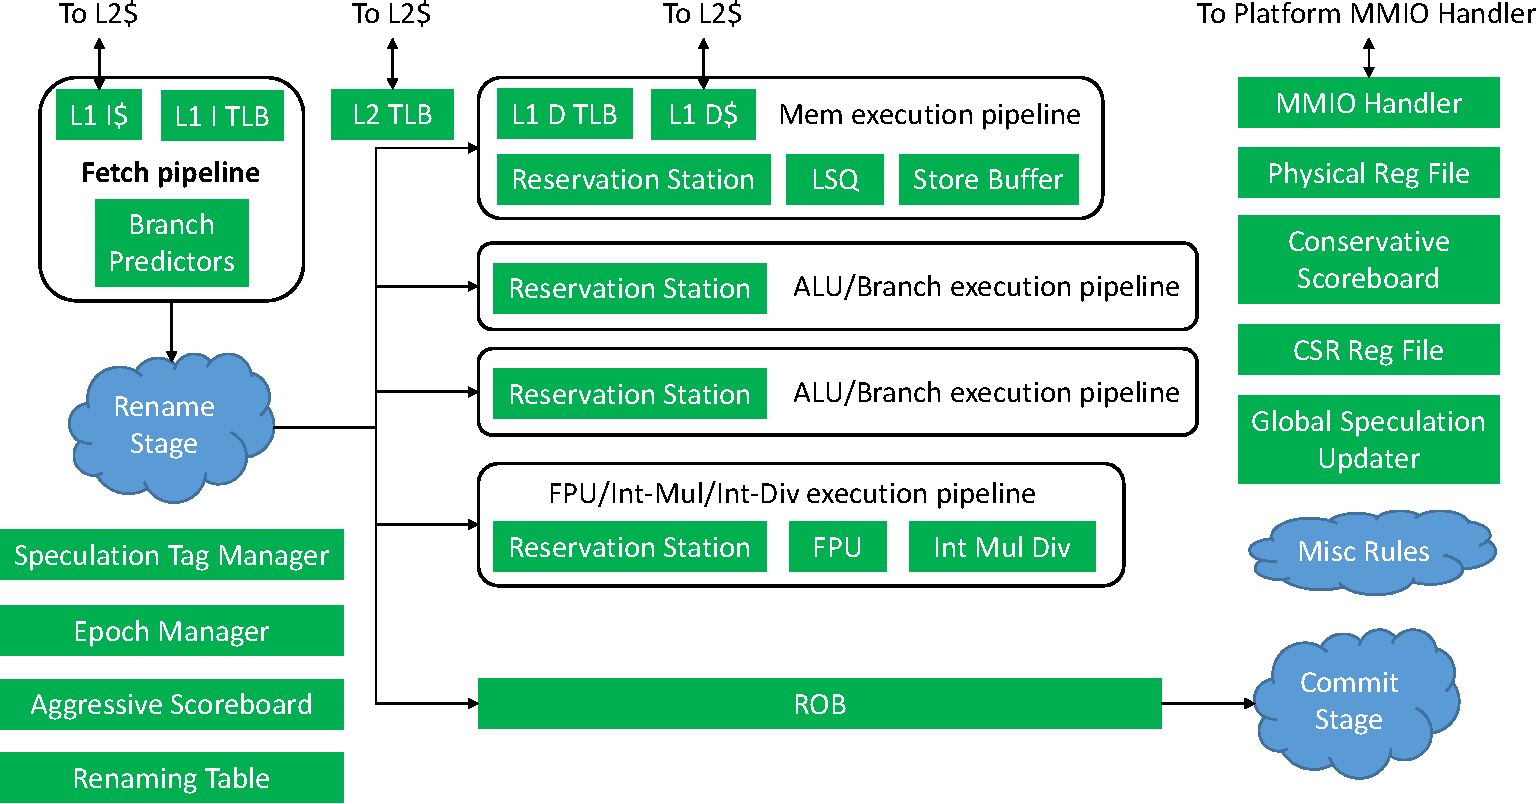
\includegraphics[width=\columnwidth]{fig/core_crop.pdf}
    \caption{Overall structure of the processor core}\label{fig:core}
\end{figure}

\noindent\textbf{Scheduling Convention:}
Since there are many modules in the core, assigning conflict matrices to different module interfaces to maximize the concurrency of rules can be difficult.
To simplify the problem, we following the convention of \emph{reverse pipeline ordering} in assigning conflict matrices.
\emph{That is, rules representing later stages in the processor pipeline (e.g., commit) are ordered before rules representing earlier stages (e.g., rename), and thus, interface methods called in later stages are ordered before methods called in earlier stages.}

Another principle in scheduling is to have common rules fire concurrently.
\emph{It is ok to have uncommon rules (e.g., mis-speculation) conflict with each other and even common rules.}

\noindent\textbf{System Instructions:}
Some instructions can change the context of the processor and are difficult to be executed out of order or concurrently with other instructions.
These instructions are called \emph{system instructions}, and include the following instructions:
\begin{itemize}
    \item \inst{ECALL} which makes a system call,
    \item \inst{EBREAK} which traps for debugger,
    \item \inst{SRET} and \inst{MRET} which return from trap handling,
    \item \inst{SFENCE.VMA} which flushes the TLBs, and
    \item \inst{FENCE.I} which is used for self-modifying code.
\end{itemize}
System instructions are executed in a blocking way, i.e., the instruction will be the only instruction in the ROB.


\noindent\textbf{Detecting Interrupt:}
We detect interrupts at \emph{rename} stage (instead of commit stage).
When an interrupt is detected, the current instruction at the rename stage will be turned into a special instruction which represents the interrupt.
The instruction will be entered into ROB and get processed at the commit stage.
Here we assume the fetch pipeline will keep delivering instructions to the rename stage, i.e., there is no low-power mode which turns off instruction fetch.

The benefits of detecting interrupts at rename stage is to ensure that all instructions in ROB are not affected by interrupts.
As a result, out-of-order commits may be possible, though we did not implement any out-of-order commits.

\noindent\textbf{Read-After-Write Hazards for CSRs:}
Our implementation ensures that there is no read-after-write hazards on CSRs in the processor.
CSRs can be modified by system instructions, exceptions, interrupts, and floating-point instructions.
The invariant of no read-after-write hazards on CSRs is guaranteed in the following way: at the rename stage, if we see a system instruction (i.e., \inst{CSRRW}), we enters the instruction into the ROB only if ROB is empty, and we flush the fetch pipeline at the same time.
As a result, there cannot be any hazards regarding the writes on CSRs by system instructions, exceptions or interrupts.

As for the hazards regarding the writes on CSRs by floating-point instructions.
We notice that only the \inst{CSRRW} instruction, which is a system instruction, can read the CSRs modified by floating-point instructions.
Therefore, the writes by floating-point instructions cannot cause any hazards.

It should be noted that there is no write-after-write or write-after-read hazards on CSRs, because all CSR writes are made at commit stage.

\noindent\textbf{Organization:}
In the rest of this section, we first introduce the general mechanism to control speculation in the back-end (Section~\ref{sec:specupdate}), and then describe each modules and top-level rules.

\subsection{Managing Speculative and Wrong-Path Instructions}\label{sec:specupdate}

Almost all instructions in the processor are speculative and may be at the wrong path, so we need to have some way to manage speculation and squash wrong-path instructions.
Since the front-end is in-order while the back-end is out-of-order, we use different schemes in the front-end and the back-end, and we explain each of the schemes next.

\subsubsection{Front-End}
The rename stage kills wrong-path instructions from the front-end (i.e., the fetch pipeline) based on the epoch in the \emph{epoch manager} (Section \mycomment{XXX}).
The fetch pipeline contains a copy of the epoch, and every fetched instruction will carry the epoch value.
At the rename stage, instructions with epochs not equal to the epoch value in the epoch manager are killed.
Whenever the PC register in the fetch pipeline needs to be redirected (because of branch mispredictions, exceptions, interrupts, or mis-speculative loads), the epoch in the epoch manager will be incremented either at the redirect time or slightly earlier.
When the PC in the fetch pipeline is truly redirected, the epoch copy in the fetch pipeline is also incremented.

Since there can be multiple consecutive redirections in the back-end, the epoch in the epoch manager should have multiple bits.
The epoch manager will recycle unused epoch values based on the epoch values of instructions seen at the rename stage.

\subsubsection{Back-End}
We use two approaches to perform squashes in the back-end:
\begin{enumerate}
    \item We delay the squash and redirection until the commit stage.
    At that time, we can simply kill every instruction in the back-end.
    \item We squash wrong-path instruction and redirect PC immediately when we find a redirection is needed (e.g., when a branch turns out to be mispredicted).
    The challenge is that we should squash only instruction younger than the instruction that triggers the redirection.
\end{enumerate}
We use the first approach for uncommon redirections, i.e., exceptions, interrupts, and the replay of mis-speculative loads that violate memory ordering.
We use the second approach for branch mispredictions only.
The implementation of these two approaches consists of the following three parts.

\noindent\textbf{Speculation tags and bit masks to track dependency on branches:}
To correctly kill wrong-path instructions in case of branch mispredictions, we assign a unique \emph{speculation tag} (type \code{SpecTag} in the source code) to each branch at the rename stage.
Every instruction will also be assigned with a speculation bit mask (type \code{SpecBits} in the source code) at the rename stage.
Each bit in the bit mask corresponds to a speculation tag.
If the bit is set, then the instruction should be killed in case the branch holding the speculation tag is mispredicted.
If a branch turns out to be predicted correctly, then the corresponding bit should be cleared from all instructions in the back-end. 
The \emph{speculation tag manager} (Section \mycomment{XXX}) assigns and recycles speculation tags, and also assigns speculation bit masks.

\noindent\textbf{Module interface to manipulate speculative instructions:}
Every module in the back-end that keeps speculative instructions should also keep the speculation bit mask for each instruction.
The module also needs to provide interface methods to allow top-level rules to squash speculative instructions or clear speculation bit masks.
All modules that keep speculative instructions except ROB provides the \code{SpeculationUpdate} interface in Figure~\ref{fig:specupdate-ifc}.
ROB provides the \code{ROB\_SpeculationUpdate} interface in Figure~\ref{fig:specupdate-ifc}.

In both interfaces, method \code{correctSpeculation} clears the speculation bit mask of each instruction in the module saccording to argument \code{mask}.
This method is called when a branch resolves to be predicted correctly.
Since multiple branches can be resolved (to be predicted correctly) in the same cycle, we use argument \code{mask} to encode the speculation tags of all these branches.

In both interfaces, method \code{incorrectSpeculation} squashes wrong-path instructions.
If argument \code{kill\_all} is true, then all instructions in the module are squashed.
This happens when commit stage commits an exception, or an interrupt, or a load that violates memory ordering.
Otherwise, only instructions whose speculation bit mask contains the speculation tag in argument \code{spec\_tag} will be squashed.
This happens when a branch is resolved and turns out to be mispredicted.
It should be noted that there can only be one source of squashing in each cycle.
In case of the ROB module, the third argument \code{inst\_tag} is the ROB index of the mispredicted branch.
It is used to simplify the squashing logic in ROB.

\begin{figure}
\begin{lstlisting}[caption={}]
interface SpeculationUpdate;
  method Action incorrectSpeculation(Bool kill_all, SpecTag kill_tag);
  method Action correctSpeculation(SpecBits mask);
endinterface
interface ROB_SpeculationUpdate;
  method Action incorrectSpeculation(Bool kill_all, SpecTag spec_tag, InstTag inst_tag);
  method Action correctSpeculation(SpecBits mask);
endinterface
\end{lstlisting}
\caption{Interface methods to manipulate speculation bit masks of modules that keep speculative instructions}\label{fig:specupdate-ifc}
\end{figure}

\noindent\textbf{Centralized entry point for manipulating speculative instructions:}
The commit stage or the branch-resolve rule does not call directly the \code{SpeculationUpdate} interface of every module to clear speculation bit masks or squashing instructions.
Instead, they both call the interface of the \emph{global speculation updater} (Section \mycomment{XXX}), which is the centralized entry point for manipulating speculative instructions.
The global speculation updater merges requests to clear speculation bit masks and then call the \code{correctSpeculation} method of every module.
It also arbitrate between requests to squash instructions and then call the \code{incorrectSpeculation} method of every module.
To some degree, having a centralized the entry point simplifies the broadcast logic for manipulating speculative instructions.



\subsection{Epoch Manager}

The epoch manager manages the epoch that is used to kill wrong-path instructions at the rename stage.
Each time a redirection happens, the epoch is incremented by one, so the epoch value will change as follows (\code{NumEpochs} is the number of unique epoch values):
\begin{center}
    0 $\rightarrow$ 1 $\rightarrow$ $\cdots$ $\rightarrow$ \code{NumEpochs}$-1$ $\rightarrow$ 0 $\rightarrow$ $\cdots$
\end{center}
The module also tracks the range of epoch values being used by instructions in the fetch pipeline.
The epoch cannot be incremented if the next epoch value falls within the range.
The range is updated by looking at the epochs of instructions coming out of the fetch pipeline.

\subsubsection{Interface}
Figure~\ref{fig:epoch-ifc} shows the interface of the epoch manager.
Now we explain each interface method:
\begin{itemize}
    \item Subinterface \code{checkEpoch}: provides a vector of methods for the rename stage to check if an instruction is at the wrong path.
    The input argument \code{e} is the epoch carried by the instruction.
    The method compares \code{e} with the internal epoch of the module, and returns false if the instruction is at the wrong path and should be killed.
    
    \item Subinterface \code{updatePrevEpoch}: provides a vector of methods to update the latest epoch values seen from the fetch pipeline.
    Every instruction that arrives at the rename stage (including wrong-path instructions) will call this method to help the module recycle unused epoch values.
    
    \item Method \code{incrementEpoch}: is called when PC needs to be redirect.
    This method increased the internal epoch of the module.
    The guard will be false if the next value of the epoch is not yet recycled (i.e., still being used by instructions in the fetch pipeline).
\end{itemize}

\begin{figure}
\begin{lstlisting}[caption={}]
interface EM_checkEpoch;
  method Bool check(Epoch e);
endinterface
interface EM_updatePrevEpoch;
  method Action update(Epoch e);
endinterface
interface EpochManager;
  interface Vector#(SupSize, EM_checkEpoch) checkEpoch;
  interface Vector#(SupSize, EM_updatePrevEpoch) updatePrevEpoch;
  method Epoch getEpoch;
  method Action incrementEpoch;
endinterface
\end{lstlisting}
\caption{Interface of epoch manager}\label{fig:epoch-ifc}
\end{figure}

\noindent\textbf{Conflict Matrix:}
The conflict matrix of the interface methods is:
\begin{enumerate}
    \item \code{checkEpoch} $<$ \code{incrementEpoch}
    \item \code{updatePrevEpoch} CF \{\code{checkEpoch}, \code{incrementEpoch}\}
\end{enumerate}
We make method \code{updatePrevEpoch} conflict free with other methods, because the recycle of unused epoch values does not need to happen immediately.

\subsubsection{Implementation}
The module has two internal registers \code{curr\_epoch} and \code{prev\_checked\_epoch}.
\code{curr\_epoch} is the current epoch value which is used to kill wrong-path instructions at the rename stage.
\code{prev\_checked\_epoch} is the last seen epoch value from the fetch pipeline.
Thus, the range of epoch values being used is: \code{prev\_checked\_epoch}, \code{prev\_checked\_epoch}$+1$, $\ldots$, \code{curr\_epoch}.

Methods \code{checkEpoch} and \code{incrementEpoch} access directly the registers.
For subinterface \code{updatePrevEpoch}, we first capture its arguments in wires, and then update the \code{prev\_checked\_epoch} register.
Wires are ok because \code{updatePrevEpoch} is conflict free with other methods.

\subsubsection{Source Code}
See module \code{mkEpochManager} in \code{//procs/lib/EpochManager.bsv}.        


\subsection{Speculation Tag Manager}\label{sec:spectag}

The speculation tag manager manages all the speculation tags (including both assigned tags and free tags).
Speculation tags are checked out or assigned at rename stage, and freed when the branch resolves in the ALU execution pipeline.
It should be noted that if a branch is mispredicted, then the speculation tags of itself and younger branches are all freed.
Since the module tracks all the in-flight speculation tags, it also assigns speculation bit mask to each instruction at the rename stage.

\subsubsection{Interface}

Figure~\ref{fig:spectag-ifc} shows the interface of the speculation tag manager.
Now we explain each interface method:
\begin{itemize}
    \item Method \code{currentSpecBits}: returns the speculation bit mask that should be assigned to the instruction at the rename stage.
    
    \item Method \code{nextSpecTag}: returns the speculation tag to be checked out for a new branch instruction at the rename stage.
    The guard is false if all tags have been checked out.
    
    \item Method \code{claimSpecTag}: checks out a new speculation tag for a new branch instruction at the rename stage.
    The guard is false if all tags have been checked out.
    
    \item Method \code{canClaim}: returns the guard of methods \code{nextSpecTag} and \code{claimSpecTag}.
    
    \item Subinterface \code{specUpdate}: See Section~\ref{sec:specupdate}.
\end{itemize}

\begin{figure}
\begin{lstlisting}[caption={}]
interface SpecTagManager;
  method SpecBits currentSpecBits;
  method SpecTag  nextSpecTag;
  method Action   claimSpecTag;
  method Bool     canClaim;
  interface SpeculationUpdate specUpdate;
endinterface
module mkSpecTagManager(SpecTagManager);
  // module implementation
endmodule
\end{lstlisting}
\caption{Interface of speculation tag manager}\label{fig:spectag-ifc}
\end{figure}

\noindent\textbf{Conflict Matrix:}
The conflict matrix of the interface methods is:
\begin{itemize}
    \item \{\code{currentSpecBits}, \code{nextSpecTag}, \code{canClaim}\} $<$ \code{claimSpecTag} $<$ \code{correctSpeculation}
    \item \{\code{currentSpecBits}, \code{nextSpecTag}, \code{canClaim}\} $<$ \code{incorrectSpeculation}
    \item \code{claimSpecTag} C \code{incorrectSpeculation}
\end{itemize}
We make \code{claimSpecTag} conflict with \code{incorrectSpeculation}, because the \code{claimSpecTag} must be called by a wrong-path instruction if \code{incorrectSpeculation} is called in the same cycle.

\subsubsection{Implementation}
The module uses EHR \code{current\_spec\_bits\_ehr} to keep the current speculation bit mask.
Each bit in the mask represents if the corresponding speculation tag is held of an in-flight branch in the ROB.
The module uses a vector of registers \code{dependent\_checkpoints} to track the dependencies between speculation tags.
\code{dependent\_checkpoints[t]} is the speculation bit mask that encodes all the speculation tags that is checked out after speculation tag \code{t} (including \code{t} also).
That is, if the branch with speculation tag \code{t} is mispredicted, then all speculation tags encoded in \code{dependent\_checkpoints[t]} should be freed.

All methods access the EHR or registers directly according to the conflict matrix.
We manually create a conflict between \code{claimSpecTag} and \code{incorrectSpeculation}.

\subsubsection{Source Code}
See module \code{mkSpecTagManager} in \code{//procs/lib/SpecTagManager.bsv}.


\subsection{Global Speculation Updater}\label{sec:globalspec}

The global speculation updater is the centralized point for calling the \code{SpeculationUpdate} interface of every module.

\subsubsection{Interface}
Figure~\ref{fig:globalspec-ifc} shows the interface of the module.
The module takes in two interface arguments.
Argument \code{ifc} is the aggregated interface of the \code{SpeculationUpdate} interface of every module.
That is, calling any method in \code{ifc} is effectively calls the corresponding method in the \code{SpeculationUpdate} interface of every module.
Argument \code{rob} is the \code{ROB\_SpeculationUpdate} method of ROB (Sections~\ref{sec:specupdate}).
The two arguments together contain all the interface methods to squash all the speculative instructions and clear all the speculation bit masks.
Now we explain each interface method returned by the module:
\begin{itemize}
    \item Subinterface \code{correctSpec}: provides a vector of methods to clear bits in every speculation bit mask in the back-end.
    This method is called when branch resolves to be predicted correctly.
    Having a vector of methods allows multiple branches to be resolved in one cycle.
    \item Method \code{incorrectSpec}: squashes speculative instructions by calling the\\ \code{incorrectSpeculation} method of every module in the back-end.
\end{itemize}

\begin{figure}
\begin{lstlisting}[caption={}]
interface GlobalSpecUpdate#(numeric type correctSpecPortNum, numeric type conflictWrongSpecPortNum);
  interface Vector#(correctSpecPortNum, Put#(SpecTag)) correctSpec;
  method Action incorrectSpec(Bool kill_all, SpecTag spec_tag, InstTag inst_tag);
endinterface
module mkGlobalSpecUpdate#(
  SpeculationUpdate ifc, ROB_SpeculationUpdate rob
)(GlobalSpecUpdate#(correctSpecPortNum, conflictWrongSpecPortNum));
  // module implementation
endmodule
\end{lstlisting}
\caption{Interface of global speculation updater}\label{fig:globalspec-ifc}
\end{figure}

\noindent\textbf{Conflict Matrix:}
The conflict matrix of the interface methods is:
\begin{itemize}
    \item \code{correcSpec[i]} CF \code{correctSpec[j]}
    \item \code{correctSpec} C \code{incorrectSpec}
    \item \code{incorrectSpec} C \code{incorrectSpec}
\end{itemize}
Note that method \code{incorrectSpec} is conflict with itself, so there can only be one rule calling it to squash instructions in each cycle.

There is no very specific reason for making \code{correctSpec} conflict with \code{incorrectSpec}.
Making conflicting may reduce the amount of data being broadcast, otherwise we need to broadcast \code{SpecBits} for both \code{correctSpec} and \code{incorrectSpec}.
Making them conflict might also simplify overall scheduling.

\subsubsection{Implementation}\label{sec:globalspec:impl}
The \code{incorrectSpec} method simply calls the \code{incorrectSpeculation} method in module argument \code{ifc} and \code{rob} (in Figure~\ref{fig:globalspec-ifc}).
The \code{correctSpec} methods use wires to record their input arguments, i.e., the speculation tag to be freed.
Then, a canonicalize rule  merges all the speculation tags that are freed into a speculation bit mask and calls the \code{correctSpeculation} method in module argument \code{ifc} and \code{rob}.
We manually create conflict between \code{correctSpec} and \code{incorrectSpec}.

Currently, the \code{incorrectSpec} and \code{correctSpec} methods will broadcast to all modules in a single cycle.
This may complicate routing.
To reduce the pressure on routing, we can broadcast these methods to modules in multiple cycles (e.g., via a register pipeline).
However, we still need to make sure that the \code{correctSpeculation} or \code{incorrectSpeculation} method of all modules are called atomically in one rule.
Futhermore, when a \code{incorrectSpec} method call is being broadcast to all the modules, we should block any future calls to this module until the broadcast is done.
This is because the instruction that initiate the future call may be killed by the broadcast.

\subsubsection{Source Code}
See module \code{mkGlobalSpecUpdate} in \code{//procs/lib/GlobalSpecUpdate.bsv}.

\subsubsection{Future Improvement}
We should pipeline the broadcast as described in Section~\ref{sec:globalspec:impl}.


\subsection{Speculative FIFO}\label{sec:specfifo}

Each entry in the speculative FIFO carries a speculation bit mask (\code{SpecBits}), and the entry will be dropped if speculation is wrong.
This FIFO is often used as FIFOs between pipeline stages in the backend.

\subsubsection{Interface}

Figure~\ref{fig:specfifo-ifc} shows the interface of this module.
The interface here has been adapted slightly from what is in the source code.
Type \code{ToSpecFifo} is the content in a speculative FIFO, i.e., a payload field \code{data} and the speculation bit mask \code{spec\_bits}.
The type of the payload is parameterized by type parameter \code{t}.
Now we explain each interface method:
\begin{itemize}
    \item Methods \code{enq}, \code{deq} and \code{first}: are the common FIFO interface methods.
    It should be noted that wrong-path entries killed by mis-speculations will not show up in the dequeue port because they are already dropped.
    \item Subinterface \code{specUpdate}: manipulates speculative states (Section~\ref{sec:specupdate}).
\end{itemize}
If the module parameter \code{lazyEnq} is true, then method \code{deq} does not affect the guard of method \code{enq}, i.e., method \code{enq} cannot claim the dequeuing entry.

\begin{figure}[t]
\begin{lstlisting}[caption={}]
typedef struct {
  t data;
  SpecBits spec_bits;
} ToSpecFifo#(type t) deriving(Bits, Eq, FShow);
interface SpecFifo#(numeric type size, type t);
  method Action enq(ToSpecFifo#(t) x);
  method Action deq;
  method ToSpecFifo#(t) first;
  interface SpeculationUpdate specUpdate;
endinterface
module mkSpecFifo#(Bool lazyEnq)(SpecFifo#(size, t));
  // module implementation
endmodule
\end{lstlisting}
\caption{Interface of speclative FIFO}\label{fig:specfifo-ifc}
\end{figure}

\noindent\textbf{Conflict Matrix:}
The conflict matrix of the interface methods is:
\begin{itemize}
    \item \code{deq} $<$ \code{enq} $<$ \code{correctSpeculation}
    \item \code{incorrectSpeculation} $<$ \code{correctSpeculation}
    \item \code{incorrectSpeculation} C \code{enq}
    \item \code{deq} C \code{incorrectSpeculation}, or \code{deq} $<$ \code{incorrectSpeculation}
\end{itemize}
It should be noted that we have implemented with versions of the FIFO.
The only difference is in the ordering between method \code{deq} and  method \code{incorrectSpeculation}.

\subsubsection{Implementation}
For each FIFO entry, we use EHRs to store the valid bit, payload, and speculation bit mask.
Methods access EHRs using the appropriate ports according to the conflict matrix.
Method \code{incorrectSpeculation} will reset the valid bit of wrong-path entries, and thus leaves holes inside the FIFO.
There is an internal rule \code{canon\_deqP} which removes the head of the FIFO if the head is an invalid entry caused by mis-speculation.
Method \code{deq} and rule \code{canon\_deqP} are mutually exclusive.

If the module parameter \code{lazyEnq} (Figure~\ref{fig:specfifo-ifc}) is true, then the guard of method \code{enq} is computed using the wire which is set using port 0 of all EHRs.
This cuts off the path from method \code{deq} to \code{enq}.

\subsubsection{Future Improvement}
Although the guard of method \code{enq} can be independent from method \code{deq}, we still need to order \code{deq} $<$ \code{enq} because of double writes on the valid bits, which cannot really happen if \code{lazyEnq} is true.
This method ordering actually complicates the internal implementation of LSQ (see Section~\ref{sec:lsq})
We should be able to design a speculative FIFO with \code{deq} CF \code{enq}.

\subsubsection{Source Code}
See module \code{mkSpecFifo} in \code{//procs/procs/lib/SpecFifo.bsv}.


\subsection{Speculative Poisoned FIFO}\label{sec:specpoisonfifo}

Entries in the speculative poisoned FIFO carry speculation bit masks, but they are marked as \emph{poisoned} instead of being dropped when mis-speculation happens.
This is commonly used skid FIFOs in parallel with in-order functional pipelines that we don't know details, e.g., the floating point pipeline.

\subsubsection{Interface}
Figure~\ref{fig:specpoisonfifo-ifc} shows the interface of the speculative poisoned FIFO (type \code{ToSpecFifo} has been explained in Figure~\ref{fig:specfifo-ifc}).
Now we explain each interface method:
\begin{itemize}
    \item Methods \code{enq}, \code{deq} and \code{first}: are the common FIFO interface methods.
    \item Method \code{first\_poisoned}: returns if the head of FIFO is poisoned or not.
    \item Subinterface \code{specUpdate}: See Section~\ref{sec:specupdate}.
\end{itemize}
If the module parameter \code{lazyEnq} is true, then method \code{deq} does not affect the guard of method \code{enq}, i.e., method \code{enq} cannot claim the dequeuing entry.

\begin{figure}[t]
\begin{lstlisting}[caption={}]
interface SpecPoisonFifo#(numeric type size, type t);
  method Action enq(ToSpecFifo#(t) x);
  method Action deq;
  method ToSpecFifo#(t) first_data;
  method Bool first_poisoned;
  interface SpeculationUpdate specUpdate;
endinterface
module mkSpecPoisonFifo#(Bool lazyEnq)(SpecPoisonFifo#(size, t));
  // module implementation
endmodule
\end{lstlisting}
\caption{Interface of speculative poisoned FIFO}\label{fig:specpoisonfifo-ifc}
\end{figure}

\noindent\textbf{Conflict Matrix:}
The conflict matrix of the interface methods is:
\begin{itemize}
    \item \code{deq} $<$ \code{enq} $<$ \code{correctSpeculation}
    \item \code{incorrectSpeculation} $<$ \code{correctSpeculation}
    \item \code{incorrectSpeculation} C \code{enq}
    \item \code{deq} $<$ \code{incorrectSpeculation}
\end{itemize}

\subsubsection{Implementation}
We use EHRs to store the fields for each FIFO entry.
Methods access EHRs using the appropriate ports according to the conflict matrix.

If the module parameter \code{lazyEnq} (Figure~\ref{fig:specfifo-ifc}) is true, then the guard of method \code{enq} is computed using the wire which is set using port 0 of all EHRs.
This cuts off the path from method \code{deq} to \code{enq}.

\subsubsection{Source Code}
See module \code{mkSpecPoisonFifo} in \code{//procs/procs/lib/SpecPoisonFifo.bsv}.


\subsection{Aggressive (Optimistic) Scoreboard}\label{sec:sbaggr}

The aggressive scoreboard holds an optimistic version of the presence bits of all the physical registers.
Instructions in the execution pipeline can optimistically set the presence bits in this scoreboard even when the instruction has not yet finished execution (but it may be close to finish).
The renaming stage will check the presence bits from this scoreboard for the source registers of the renaming instruction, and unset the present bit in this scoreboard for the destination register of the renaming instruction.

The interface and module presented here are slightly different from what is the source code, because the module in the source code is used for not only this aggressive scoreboard but also another conservative scoreboard (Section~\ref{sec:prf+sbcons}).

\subsubsection{Interface}
Figure~\ref{fig:aggr-sb-ifc} shows the interface of this module.
Now we explain each interface method: 
\begin{itemize}
    \item Subinterface \emph{setReady}: provides a vector of methods for instructions in execution pipelines to set the presence bits of their physical destination registers optimistically.
    \item Subinterface \emph{eagerLookup}: provides a vector of methods for instructions at the renaming stage to check the presence bits of their physical source registers.
    \item Subinterface \emph{setBusy}: provides a vector of methods for instructions at the renaming stage to unset the presence bits of their physical destination registers.
\end{itemize}

\begin{figure}
\begin{lstlisting}[caption={}]
// PhyRegs is a struct containing all the physical regs of an instruction
// RegsReady is a struct containing the presence bits for all the physical regs of an instruction
// PhyRIndex is the index of a physical reg
// SupSize is the superscalar size
interface SbLookup;
  method RegsReady get(PhyRegs r);
endinterface
interface SbSetBusy;
  method Action set(Maybe#(PhyRIndx) dst);
endinterface
interface ScoreboardAggr#(numeric type setReadyNum);
  interface Vector#(setReadyNum, Put#(PhyRIndx)) setReady;
  interface Vector#(SupSize, SbLookup) eagerLookup;
  interface Vector#(SupSize, SbSetBusy) setBusy;
endinterface
module mkScoreboardAggr(ScoreboardAggr#(setReadyNum));
  // module implementation
endmodule
\end{lstlisting}
\caption{Interface of the aggressive scoreboard}\label{fig:aggr-sb-ifc}
\end{figure}

\noindent\textbf{Conflict Matrix:}
The conflict matrix of the interface methods is:
\begin{center}
    setReady[0] $<$ $\cdots$ $<$ setReady[setReadyNum-1] $<$ eagerLookup[0] $<$ setBusy[0] $<$ eagerLookup[1] $<$ setBusy[1] $<$ $\cdots$ $<$ eagerLookup[SupSize-1] $<$ setBusy[SupSize-1].
\end{center}
We put all methods in a total order, though the conflict matrix does not need to transitive.
We order setReady $<$ eagerLookup to match the rule ordering between instruction-execution rules (which call setReady) and the renaming rule (which calls eagerLookup).
The rule ordering is because the execution rules are in later stages of the pipeline than renaming.
Thus, eagerLookup will observe the effects of all the calls to setReady in the same cycle, and this is why we call it ``eager''.
Methods eagerLookup[$i$] and setBusy[$i$] are used by the $i^{th}$ renamed instruction at the renaming stage in each cycle.
Since the $i^{th}$ instruction should see the renaming effects of all previous instructions, we order setBusy[$0\ldots i-1$] $<$ eagerLookup[$i$].

\subsubsection{Implementation}
The implementation of the module does not contain any internal rules.
It just uses a vector of EHRs to hold the presence bits, one EHR for each bit.
The interface methods access the EHRs using the appropriate port according to the conflict matrix.

\subsubsection{Source Code}
See the followings:
\begin{itemize}
    \item module \texttt{mkScoreboardAggr} in \texttt{//procs/RV64G\_OOO/ScoreboardSynth.bsv}, and
    \item module \texttt{mkRenamingScoreboard} in file \texttt{//procs/lib/Scoreboard.bsv}.
\end{itemize}
  

\subsection{Physical Register File and Conservative Scoreboard}\label{sec:prf+sbcons}

The physical register file contains the value for each physical register, and the conservative scoreboard contains the presence bit for each physical-register value.
Instructions at the renaming stage will unset the presence bits of the destination physical registers.
Instructions that just finish execution write data into the physical register file and set the presence bits simultaneously.
Instructions in the execution pipeline read both the physical register file and the scoreboard to get the source operand and whether the operand data is present or not.
The scoreboard is called conservative because each presence bit is set only when the data is written to the corresponding physical register.

Although the physical register file and the conservative scoreboard are currently implemented as two separate modules, we describe them as one module here because they should be accessed together.

\subsubsection{Interface}
Figure~\ref{fig:prf-sb-ifc} shows the interface of the fused module of the physical register file and the conservative scoreboard.
It should be noted that the interface shown here is different from what is in the source code, which splits this module as two separate modules.

\begin{figure}[!htb]
\begin{lstlisting}[caption={}]
// PhyRIndex is the index of a physical reg
// SupSize is the superscalar size
interface RFileWr;
  method Action wr(PhyRIndx rindx, Data data);
endinterface
interface RFileRd;
  method Maybe#(Data) rd1(PhyRIndx rindx);
  method Maybe#(Data) rd2(PhyRIndx rindx);
  method Maybe#(Data) rd3(PhyRIndx rindx);
endinterface
interface SbSetBusy;
  method Action set(Maybe#(PhyRIndx) dst);
endinterface
interface RFileSbCons#(numeric type wrNum, numeric type rdNum);
  interface Vector#(wrNum, RFileWr) write;
  interface Vector#(rdNum, RFileRd) read;
  interface Vector#(SupSize, SbSetBusy) setBusy;
endinterface
module mkRFileSbCons(RFileSbCons#(wrNum, rdNum));
  // module implementation
endmodule
\end{lstlisting}
\caption{Interface of physical register file and conservative scoreboard}\label{fig:prf-sb-ifc}
\end{figure}

Now we explain each interface method:
\begin{itemize}
    \item Subinterface \emph{write}: provides a vector of methods for instructions that just finish execution to write the data into the physcial register file and set the presence bit.
    \item Subinterface \emph{read}: provides a vector of methods for instructions at register-read stage to read both the data and presence bit of the source register.
    In case the presence bit is unset, the method returns \texttt{Invalid}.
    \item Subinterface \emph{setBusy}: provides a vector of methods for instructions at the renaming stage to unset the presence bits of their physical destination registers.
    this method will be called together with the one in the aggressive scoreboard.
\end{itemize}

The conflict matrix of the interface methods is:
\begin{itemize}
    \item read CF \{write, setBusy\}
    \item write[0] $<$ write[1] $<$ $\cdots$ $<$ write[wrNum-1] $<$ setBusy[0] $<$ setBusy[1] $<$ $\cdots$ $<$ setBusy[wrNum-1]
\end{itemize}
We set all the read methods conflict free with all the write methods, because reads do not need to reflect the effects of writes immediately.
In case an old instruction is writing a register which is being read by a younger instruction as a source operand, it is ok for the read method to return \texttt{Invalid} even if the write method has been called.
This simply delays the execution of the younger instruction.
In our implementation, the read method will return \texttt{Invalid} if a write for the same physical register is being performed in the same cycle.
This can cut off the combinational path.

Forcing read methods to be ordered before write methods can cause rule-scheduling problems, because rules that read the register file are in earlier pipeline stages than rules that write register file.
That is, the method ordering will not agree with the (desired) top-level rule ordering.

We also set all the read methods conflict free with all the setBusy methods.
This is because the renaming algorithm guarantees that a physical register that is being used as a source operand of a (currently correct-path) instruction cannot be a free register for renaming destination architectural registers.
However, \emph{it is still desirable in the furture implementation to set all the read methods $<$ all the setBusy methods}, because reads happen in later pipeline stages than setBusy does.

We order all the write methods before all the setBusy methods, because write methods are called in later stages in the pipeline than setBusy methods.

\subsubsection{Implementation}
The implementation uses a vector of EHRs to store the register data, and another vector of EHRs to store the presence bits.
The write methods and set busy methods directly access the EHRs using appropriate ports according to the conflict matrix of the interface.

The read methods do not directly access the EHRs.
We use a vector of wires to retrieve value of port 0 of each EHR, and the read methods read from these wires.
This prevents any combinational path from write to read.
This is a valid implementation because the read methods are conflict free with the write and setBusy methods, and the read methods can safely ignore the effects caused by the write or setBusy methods.

\subsubsection{Source Code}
See the followings:
\begin{itemize}
    \item module \texttt{mkRFileSynth} in file \texttt{//procs/RV64G\_OOO/RFileSynth.bsv},
    \item module \texttt{mkRFile} in file \texttt{//procs/lib/PhysRFile.bsv},
    \item module \texttt{mkScoreboardCons} in file \texttt{//procs/RV64G\_OOO/ScoreboardSynth.bsv}, and
    \item module \texttt{mkRenamingScoreboard} in file \texttt{//procs/lib/Scoreboard.bsv}.
\end{itemize}

\subsubsection{Future Improvement}
There are two improvements to make in a future implementation:
\begin{enumerate}
    \item Merge the physical register file and the conservative scoreboard into one module to ensure that their methods are called together.
    \item Order the read methods before the setBusy methods, so we don't need to rely on the high-level invariant of the renaming algorithm to ensure correctness.
\end{enumerate}

\subsection{Renaming Table}\label{sec:rt}

The renaming table manages the mapping from architectural registers to physical registers.
The rename stage queries it to get the physical registers for the source registers of instructions and rename the destination registers of the instructions.
The commit stage calls it to recycle unused physical registers.
On mis-speculation, the renaming table also needs to be recovered.

\subsubsection{Interface}

Figure~\ref{fig:rt-ifc} shows the interface of the renaming table.
Now we explain each interface:
\begin{itemize}
    \item Subinterface \code{rename}: provides a vector of methods to be called by instructions at the rename stage.
    \begin{itemize}
        \item Method \code{getRename}: returns the physical registers of the give source architectural registers according to the current mapping.
        \item Method \code{claimRename}: claims a free physical register to rename the give destination architectural register and updates the mapping.
        \item Method \code{canRename}: returns the guard of \code{claimRename}.
    \end{itemize}
    \item Subinterface \code{commit}: provides a vector of methods to be called by instructions at the commit stage.
    \begin{itemize}
        \item Method \code{commit}: recycles the physical register that is overshadowed by the renaming made by the committing instruction.
        \item Method \code{canCommit}: returns the guard of \code{commit}.
    \end{itemize}
    \item Subinterface \code{specUpdate}: manipulates speculative states (Section~\ref{sec:specupdate}).
\end{itemize}
\emph{We assume every instruction will call method \code{claimRename} at the the rename stage.}
Even if the instruction does not have a destination register, it will claim a physical register.
This simplifies the implementation of superscalar rename and commit.

\begin{figure}
\begin{lstlisting}[caption={}]
interface RTRename;
  method PhyRegs getRename(ArchRegs r);
  method Action claimRename(ArchRegs r, SpecBits sb);
  method Bool canRename;
endinterface
interface RTCommit;
  method Action commit;
  method Bool canCommit;
endinterface
interface RegRenamingTable;
  interface Vector#(SupSize, RTRename) rename;
  interface Vector#(SupSize, RTCommit) commit;
  interface SpeculationUpdate specUpdate;
endinterface
module mkRegRenamingTable(RegRenamingTable);
  // module implementation
endmodule
\end{lstlisting}
\caption{Interface of the renaming table}\label{fig:rt-ifc}
\end{figure}

\noindent\textbf{Conflict Matrix:}
The conflict matrix of the interface methods is:
\begin{itemize}
    \item \code{commit[0]} $<$ \code{commit[1]} $<$ $\cdots$ $<$ \code{commit[SupSz-1]} $<$ \code{rename[0].getRename} $<$ \\ \code{rename[0].claimRename} $<$ \code{rename[1].getRename} $<$ \code{rename[1].claimRename} $<$ $\cdots$ $<$ \code{rename[SupSize-1].getRename} $<$ \code{rename[SupSize-1].claimRename}
    \item \code{incorrectSpeculation} $<$ \code{correctSpeculation}
    \item \code{commit} $<$ \code{incorrectSpeculation}
    \item \code{incorrectSpeculation} C \code{rename.claimRename}
\end{itemize}
We order \code{rename[0].claimRename} before \code{rename[1].getRename}, because the second instruction renamed at the rename stage should see the effects made by the first instruction renamed at the rename stage in the same cycle.

\subsubsection{Implementation}
We keep the renaming mapping made by committed instructions as a table, and keep all the renamings made by in-flight instructions in ROB as a FIFO of deltas.
We did not use EHRs in this implementation.
The bypass is limited only between superscalar renamings.
We choose to use wires to capture all the method arguments, process all the actions in a canonicalization rule, explicitly bypass values from \code{claimRename} methods to \code{getRename} methods, and artificially creates method orderings.
It should be noted that \code{getRename} methods can ignore the effects of \code{commit} methods which do not change the renaming mapping.
This is a major reason not to use EHRs.

\subsubsection{Source Code}
See module \code{mkRegRenamingTable} in \code{//procs/lib/RenamingTable.bsv}.


\subsection{ROB}\label{sec:rob}

The ROB keeps all the in-flight instructions that have been renamed but not committed.
Instructions are enqueued into ROB in order at the renaming stage, and are dequeued from the ROB in order at the commit stage.
Instructions in the execution pipeline will also access the corresponding ROB entry.

\subsection{Interface}
Before introducing the interface of the module, we first explain the fields in an ROB entry.
Figure~\ref{fig:rob-entry} shows the definition of type ToReorderbuffer which is a struct that contains all the fields in an ROB entry.
Now we explain each field (``the instruction'' refers to the instruction in the ROB entry):
\begin{itemize}
    \item \emph{pc}: is the PC of the instruction.
    It is set when the renaming stage enqueues the instruction into ROB.
    \item \emph{iType}: is the type (e.g., ALU, load, store, etc.) of the instruction.
    It is set when the renaming stage enqueues the instruction into ROB.
    \item \emph{csr}: is the CSR index to access if the instruction is a CSRRW instruction.
    It is set when the renaming stage enqueues the instruction into ROB.
    \item \emph{claimed\_phy\_reg}: is true if the instruction has claimed a physical register to rename a architectural register.
    It is set when the renaming stage enqueues the instruction into ROB.
    If this field is true, then the instruction needs to release the originally mapped physical register for the renamed architectural register at commit stage.
    This field is always true unless the instructions represents an interrupt (we detect interrupts at renaming stage and encode an interrupt as an instruction in ROB) or the instruction has got an exception before being enqueued into ROB.
    \item \emph{trap}: is the exception or interrupt associated with the instruction.
    It is set when the renaming stage enqueues the instruction into ROB, or when the memory instruction is dequeued from LSQ and it has triggered a memory page fault (or memory access fault) before.
    \item \emph{ppc\_vaddr\_csrData}: is a tagged union.
    The field is initially set to the predicted next PC when the instruction is enqueued into ROB at the renaming stage.
    If the instruction is a memory instruction, then the field will be set to the virtual memory address after address translation.
    The virtual address will be used at the commit stage if the instruction triggers a page fault or access fault.
    If the instruction is a CSRRW instruction that performs a read-modify-write on an CSR, then the field will be set to the original value of the CSR when the instruction leaves the ALU execution pipeline.
    If the instruction is a branch instruction, then the field will set to the computed next PC when the instruction leaves the ALU execution pipeline.
    \item \emph{fflags}: is the status flags (e.g., overflow and underflow) of the FPU computation performed by the instruction in case the instruction is an FPU instruction.
    It is set when the FPU computation is done in the execution pipeline.
    It will be used at the commit stage to update an CSR for FPU.
    \item \emph{will\_dirty\_fpu\_state}: is true if the destination register of the instruction is an floating point register.
    It is set when the instruction is enqueued into ROB at the renaming stage.
    It will be used at the commit stage to update an CSR for FPU.
    \item \emph{rob\_inst\_state}: is a single bit to represent if the instruction has finished execution or not.
    \item \emph{lsqTag}: is the index to LSQ if the instruction is a memory or fence instruction.
    \item \emph{ldKilled}: is true if the instruction is a load which is killed because the load speculation violates store-to-load memory dependency or memory ordering required by the consistency model.
    It is set when the load instruction is dequeued from LSQ.
    \item \emph{memAccessAtCommit}: is true if the memory instruction must be executed non-speculatively, i.e., the instruction, an MMIO or an atomic (i.e., load-reserve, store-conditional and read-modify-write).
    It is set when the instruction finishes translating address.
    If this field is true, the instruction needs to notify LSQ when the instruction reaches the commit slot of the ROB (i.e., becomes the oldest in ROB).
    LSQ can issue this instruction to memory only after receiving the notification.
    \item \emph{lsqAtCommitNotified}: is true if the instruction has already notified LSQ about reaching the commit slot of ROB.
    (This field is meaningful only if the memAccessAtCommit field is true.)
    It prevents repeated notifications to the LSQ.
    It is set when the notification to LSQ happens.
    \item \emph{nonMMIOStDone}: is true if the instruction is a non-MMIO store and has translated its address and has computed its data, i.e., the store can be considered as executed even though it has not been issued to memory.
    If this field is true, then the instruction needs to notify LSQ when it is dequeued from ROB at the commit stage.
    (The lsqAtCommitNotified field does not need to be set because the entry is already dequeued from ROB.)
    This field is set when the instruction finishes translating address.
    \item \emph{epochIncremented}: is true if the instruction has incremented the epoch at the renaming stage to drop any future instructions from the fetch stage.
    This field is true only when the instruction represents an interrupt, is a system instruction that needs to be performed in a blocking way, or triggers an exception before being enqueued into ROB.
    If this field is true, then when this instruction is committed, the commit stage does not need to increment the epoch at the renaming stage again when redirecting the fetch stage (the epoch at the fetch stage still needs to be incremented).
    This field is set when the renaming stage enqueues the instruction into ROB.
    \item \emph{spec\_bits}: is the bit mask to encode all the older unresolved branches, i.e., the misprediction of any such branches will kill this instruction.
    This field is set when the renaming stage enqueues the instruction into ROB.
\end{itemize}

\begin{figure}[!htb]
\begin{lstlisting}[caption={}]
typedef struct {
  Addr               pc;
  IType              iType;
  Maybe#(CSR)        csr;
  Bool               claimed_phy_reg;
  Maybe#(Trap)       trap;
  PPCVAddrCSRData    ppc_vaddr_csrData;
  Bit#(5)            fflags;
  Bool               will_dirty_fpu_state;
  RobInstState       rob_inst_state;
  LdStQTag           lsqTag;
  Maybe#(LdKilledBy) ldKilled;
  Bool               memAccessAtCommit;
  Bool               lsqAtCommitNotified;
  Bool               nonMMIOStDone;
  Bool               epochIncremented;
  SpecBits           spec_bits;
} ToReorderBuffer deriving(Bits, Eq, FShow);
\end{lstlisting}
\caption{Fields in an ROB entry}\label{fig:rob-entry}
\end{figure}

Figures~\ref{fig:rob-subifc} and \ref{fig:rob-ifc} show the interface of ROB.
The interface parameters aluExeNum and fpuMulDivExeNum are the numbers of ALU execution pipelines and FPU/Int-Multipy/Int-Divide execution pipelines, respectively.
Now we explain each method in the ROB interface (Figure~\ref{fig:rob-ifc}):
\begin{itemize}
    \item Subinterface \emph{enqPort}: 
\end{itemize}

\begin{figure}[!htb]
\begin{lstlisting}[caption={}]
// InstTag is the index of ROB entry
// ControlFlow is a struct that contains the computed next PC
// ToReorderBuffer is a struct for an ROB entry
interface ROB_EnqPort;
  method Bool canEnq;
  method Action enq(ToReorderBuffer x);
  method InstTag getEnqInstTag;
endinterface
interface ROB_DeqPort;
  method Bool canDeq;
  method Action deq;
  method InstTag getDeqInstTag;
  method ToReorderBuffer deq_data;
endinterface
interface ROB_setExecuted_doFinishAlu;
  method Action set(InstTag x, Maybe#(Data) csrData, ControlFlow cf);
endinterface
interface ROB_setExecuted_doFinishFpuMulDiv;
  method Action set(InstTag x, Bit#(5) fflags);
endinterface
interface ROB_getOrigPC;
  method Addr get(InstTag x);
endinterface
interface ROB_getOrigPredPC;
  method Addr get(InstTag x);
endinterface
\end{lstlisting}
\caption{Subinterfaces of ROB}\label{fig:rob-subifc}
\end{figure}

\begin{figure}[!htb]
\begin{lstlisting}[caption={}]
// SupSize is the superscalar size
interface SupReorderBuffer#(numeric type aluExeNum, numeric type fpuMulDivExeNum);
  interface Vector#(SupSize, ROB_EnqPort) enqPort;
  method Bool isEmpty;
  interface Vector#(SupSize, ROB_DeqPort) deqPort;
  method Action setLSQAtCommitNotified(InstTag x);
  method Action setExecuted_deqLSQ(InstTag x, Maybe#(Exception) cause, Maybe#(LdKilledBy) ld_killed);
  interface Vector#(aluExeNum, ROB_setExecuted_doFinishAlu) setExecuted_doFinishAlu;
  interface Vector#(fpuMulDivExeNum, ROB_setExecuted_doFinishFpuMulDiv) setExecuted_doFinishFpuMulDiv;
  method Action setExecuted_doFinishMem(InstTag x, Addr vaddr, Bool access_at_commit, Bool non_mmio_st_done);
  interface Vector#(TAdd#(1, aluExeNum), ROB_getOrigPC) getOrigPC;
  interface Vector#(aluExeNum, ROB_getOrigPredPC) getOrigPredPC;
  method InstTime getEnqTime;
  method Bool isEmpty_ehrPort0;
  method Bool isFull_ehrPort0;
  interface ROB_SpeculationUpdate specUpdate;
endinterface
module mkSupReorderBuffer(SupReorderBuffer#(aluExeNum, fpuMulDivExeNum);
  // module implementation
endmodule
\end{lstlisting}
\caption{Interface of ROB}\label{fig:rob-ifc}
\end{figure}



\subsection{Reservation Station}\label{sec:rs}
Reservation station is the first module of every execution pipeline.
Rename stage enters instructions into one of the reservation stations.
The module tracks whether unissued instructions are ready to issue to execution, and schedules ready instructions to issue.

\subsubsection{Interface}\label{sec:rs:ifc}
Figure~\ref{fig:rs-ifc} shows the module interface of the reservation station.
Type \code{ToReservationStation} contains all the fields in a reservation-station entry:
\begin{itemize}
    \item Field \code{data}: is the information that an instruction wants to store in the entry.
    Its type is parameterized
    \item Field \code{regs}: is the indexes of the physical registers used by the instruction.
    \item Field \code{spec\_bits}: is speculation bit mask of the instruction.
    \item Field \code{spec\_tag}: is the speculation tag of the instruction if it is a branch.
    In future implementations, this field should be moved into the \code{data} field to save area, because not all instruction need this field.
    \item Field \code{regs\_ready}: is the register presence bits of all the source registers of the instruction.
\end{itemize}
Interface \code{ReservationStation} has three type parameters:
\begin{itemize}
    \item Numeric type \code{size}: is the number of entries in the reservation station.
    \item Numeric type \code{setRegReadyNum}: is the number of concurrent wakeups.
    \item Type \code{a}: is the type parameter for \code{ToReservationStation}.
\end{itemize}
Now we explain each interface method:
\begin{itemize}
    \item Method \code{enq}: enters an instruction into the reservation station.
    \item Method \code{canEnq}: returns the guard of method \code{enq}, i.e., whether there is a free entry.
    \item Method \code{setRobEnqTime}: tells the module about the conceptual enqueue pointer of ROB.
    This information is used in the age-based scheduling policy, i.e., older instructions have higher priority in being issued.
    \item Method \code{dispatchData}: returns the ready entry that is scheduled to be issued.
    The guard is false if there is no entry to issue.
    \item Method \code{doDispatch}: removes the ready entry that is scheduled to be issued from the module.
    \item Subinterface \code{setRegReady}: provides a vector of methods to wake up instructions, i.e., a physical register becomes ready.
    \item Method \code{approximateCount}: returns the approximate number of occupied entries in the module.
    The result is used by the rename stage as a heuristic to choose which reservation station to enter an instruction if there are multiple identical execution pipelines (e.g., there can be two ALU pipelines).
    \item Subinterface \code{specUpdate}: manipulates speculative states (Section~\ref{sec:specupdate}).
\end{itemize}

\begin{figure}[t]
\begin{lstlisting}[caption={}]
typedef struct {
  a data;
  PhyRegs regs;
  InstTag tag;
  SpecBits spec_bits;
  Maybe#(SpecTag) spec_tag;
  RegsReady regs_ready;
} ToReservationStation#(type a) deriving(Bits, Eq, FShow);
interface ReservationStation#(numeric type size, numeric type setRegReadyNum, type a);
  method Action enq(ToReservationStation#(a) x);
  method Bool canEnq;
  method Action setRobEnqTime(InstTime t);
  method ToReservationStation#(a) dispatchData;
  method Action doDispatch;
  interface Vector#(setRegReadyNum, Put#(Maybe#(PhyRIndx))) setRegReady;
  method Bit#(TLog#(TAdd#(size, 1))) approximateCount;
  interface SpeculationUpdate specUpdate;
endinterface
module mkReservationStation(ReservationStation#(size, setRegReadyNum, a));
  // module implementation
endmodule
\end{lstlisting}
\caption{Interface of reservation station}\label{fig:rs-ifc}
\end{figure}

\noindent\textbf{Conflict Matrix:}
The conflict matrix of the module is:
\begin{itemize}
    \item \code{setRegReady[0]} $<$ \code{setRegReady[1]} $<$ $\cdots$ $<$ \code{setRegReady[setRegReadyNum-1]}
    \item \{\code{setRegReady}, \code{dispatchData}, \code{doDispatch}, \code{canEnq}\} $<$ \code{enq}
    \item \code{setRobEnqTime} $<$ \code{dispatchData} $<$ \code{doDispatch}
    \item \code{dispatchData} $<$ \code{incorrectSpeculation}
    \item \code{incorrectSpeculation} C \{\code{enq}, \code{doDispatch}\}
    \item \{\code{enq}, \code{dispatchData}, \code{doDispatch}, \code{incorrectSpeculation}\} $<$ \code{correctSpeculatoin}
    \item All others are conflict free.
\end{itemize}

We make \code{dispatchData} and \code{doDispatch} conflict free with \code{setRegReady}, because \code{dispatchData} and \code{doDispatch} do not need to see the effect of \code{setRegReady} in the same cycle.
An instruction can be issued many cycles after it is waken up.
This cuts off the bypass path from \code{setRegReady} to \code{dispatchData} (i.e., selecting a ready entry).

We make \code{canEnq} conflict free with \code{doDispatch}, because the reservation station does not need to have pipelined behavior, i.e., being able to remove and insert simultaneously when it is full.
This cuts off bypass from \code{doDispatch} to \code{canEnq} which is used in the rename stage.

We order \code{enq} after \code{setRegReady}, \code{dispatchData}, \code{doDispatch}, and \code{canEnq} because \code{enq} happens at the earliest stage, i.e., the rename stage.

We order \code{setRobEnqTime} before \code{dispatchData} and \code{doDispatch} because scheduling an instruction to issues uses the ROB enqueue pointer as a heuristic.

We order \code{incorrectSpeculation} conflict with \code{enq} and \code{doDispatch} to cut off any bypass paths.

We order \code{correctSpeculation} after other methods because of the convention stated in Section~\ref{sec:specupdate}.

\subsubsection{Implementation}
The module uses a set of EHRs to store an entry, i.e., one EHR per field.
The module also use a vector of EHRs to store the valid bits of each entry.
Methods \code{setRegReady}, \code{correctSpeculation} and \code{incorrectSpeculation} access the EHRs directly using EHR ports according to the conflict matrix.

Method \code{canEnq} (i.e., the guard of \code{enq}) does not check the valid bits directly.
An internal rule searches through valid bits using EHR port 0 to find an empty entry, and then set a wire with the entry index (a \code{Maybe} type).
Method \code{canEnq} checks if the wire contains a valid index.
Method \code{enq} writes to entry indexed by the wire value, but it writes to the appropriate EHR port of data fields according to the conflict matrix.

Methods \code{dispatchData} and \code{doDispatch} does not check the register-ready bits (\code{reg\_ready}) in the EHRs directly.
The module uses a vector of wires to catch the values of the register-ready bits with EHR port 0.
The methods use the values of the wires to determine which one is ready to issue.
Wires are acceptable because both \code{dispatchData} and \code{doDispatch} are conflict-free with \code{setRegReady}.
For fields other than register-ready bits, the methods access the EHRs directly using the appropriate ports.

Method \code{setRobEnqTime} uses a wire to record its argument.
And method \code{dispatchData} uses the wire value in the issue-scheduling policy.
Wire is acceptable because this is a performance feature, unrelated to correctness.

We also manually make \code{incorrectSpeculation} conflict with \code{enq} and \code{doDispatch}.

\subsubsection{Source Code}
See the followings:
\begin{itemize}
    \item module \code{mkReservationStation} in \code{//procs/lib/ReservationStationEhr.bsv},
    \item module \code{mkReservationStationAlu} in \code{//procs/RV64G\_OOO/ReservationStationAlu.bsv},
    \item module \code{mkReservationStationMem} in \code{//procs/RV64G\_OOO/ReservationStationMem.bsv}, and
    \item module \code{mkReservationStationFpuMulDiv} in\\ \code{//procs/RV64G\_OOO/ReservationStationFpuMulDiv.bsv}.
\end{itemize}

\subsubsection{Future Implementation}
We should move field \code{spec\_tag} into field \code{data} in type \code{ToReservationStation} as described in Section~\ref{sec:rs:ifc}.


\subsection{LSQ}\label{sec:lsq}

LSQ (load-store queue) keeps loads and stores.
It executes loads out of order and speculatively and keep tracks of violations of memory orderings.

Loads and stores are kept in separate queues, i.e., LQ and SQ.
LQ contains loads and load-reserves.
SQ contains stores, store-conditionals, atomic read-modify-writes, and \emph{fence instructions}.
In future, we should move Reconcile fences to LQ.

In order to observe the memory dependency between loads and stores, each load in LQ keeps track of the index of the immediately preceding SQ entry.
In case a load has been issued from LQ, the load needs to track whether its value will come from the cache or by forwarding from an SQ entry or an SB entry.
When a load tries to issue, it may not be able to proceed because of fences or partially overlapped older stores.
In such cases, the load records the source that stalls it, and retries after the source of the stall has been resolved.
In case of ROB flush, if a load, which is waiting for the memory response, is killed, then this load entry is marked as waiting for a wrong path response.
Because of this bit, we can reallocate this entry to a new load, but not issue it until the bit is cleared.

Atomic instructions (load-reserve, store-conditional and read-modify-write), MMIO accesses, and fence instructions are handled in a conservative way.
When such an instruction reaches the commit slot of the ROB, it is dequeued from LSQ and then executed.
After the execution finishes, the instruction can be committed from ROB.

We try to dequeue LQ as soon as possible to recycle this critical resource.
Dequeuing a load requires all older SQ entries cannot kill the load.
To check this, we sequentially \emph{verify} each SQ entry (from old to young) to make sure the SQ entry cannot squash a younger load.

\subsubsection{Interface}

\begin{figure}
\begin{lstlisting}[caption={}]
typedef struct {
  InstTag            instTag;
  LdQMemFunc         memFunc;
  Bool               unsignedLd;
  ByteEn             byteEn;
  Bool               acq;
  Bool               rel;
  Maybe#(PhyDst)     dst;
  Addr               paddr;
  Bool               isMMIO;
  ByteEn             shiftedBE;
  Maybe#(Exception)  fault;
  Bool               computed;
  Bool               inIssueQ;
  Bool               executing;
  Bool               done;
  Maybe#(LdKilledBy) killed;
  Maybe#(StQTag)     olderSt;
  Bool               olderStVerified;
  Maybe#(StQTag)     readFrom;
  Maybe#(LdQTag)     depLdQDeq;
  Maybe#(StQTag)     depStQDeq;
`ifndef TSO_MM
  Maybe#(LdQTag)     depLdEx;
  Maybe#(SBIndex)    depSBDeq;
`endif
  SpecBits           specBits;
  Bool               atCommit;
  Bool               waitWPResp;
} LdQEntry deriving (Bits, Eq, FShow);
\end{lstlisting}
\caption{Fields in a LQ entry}\label{fig:lq-entry}
\end{figure}

Figure~\ref{fig:lq-entry} shows the fields of a LQ entry:
\begin{itemize}
    \item Field \code{instTag}: is the ROB index of the load.
    \item Field \code{memFunc}: specifies the type of the load (i.e., load or load-reserve).
    \item Field \code{unsignedLd}: indicates if the load is unsigned or not.
    \item Field \code{byteEn}: is a bit mask that specifies the position of the useful load-data bytes in an 8B double-word.
    This bit mask is taken directly from the decode result, and is not shifted according to the address.
    For example, if the load is a load-byte, then the least significant bit of the bit mask is set regardless of the load address.
    \item Field \code{acq}: is true if the entry is a load-reserve and carries a Reconcile fence.
    \item Field \code{rel}: is true if the entry is a load-reserve and carries a Commit fence.
    \item Field \code{dst}: is the destination physical register of the load.
    \item Field \code{paddr}: is the physical address of the load.
    This field is meaningful only if field \code{computed} is true.
    \item Field \code{isMMIO}: indicates if the load is accessing MMIO region.
    This field is meaningful only if field \code{computed} is true.
    \item Field \code{shiftedBE}: specifies the position of the useful load data in an 8B double-word which is loaded from an 8B aligned address.
    This is, it is \code{byteEn} shifted according to the lower bits of the address.
    \item Field \code{fault}: records the exception happened during address translation or MMIO access.
    \item Field \code{computed}: is set true when the translated address is filled into the LQ entry.
    \item Field \code{inIssueQ}: is set true when the load is identified as able to issue (to memory or get bypass), and is unset when the load is truly issued to execution.
    \item Field \code{executing}: is set when the load is issued to execution.
    \item Field \code{done}: is set when the load result returns.
    \item Field \code{killed}: is set when the load is detected to violate memory ordering (e.g., store-to-load dependency or memory consistency).
    The load is not dropped immediately, and will be handled in a way similar to exceptions.
    The reason for the violation is also recorded for performance evaluation.
    \item Field \code{olderSt}: is the SQ index of the immediately older store than this load.
    This field is \code{Invalid} if there is no older stores in SQ.
    \item Field \code{olderStVerified}: is set true to indicate that the load can be retired from LQ, i.e., older entries in SQ should not affect the load.
    This is set by an internal rule of the module.
    \item Field \code{readFrom}: records the source of the load result when the load starts execution.
    This field is meaningful only if field \code{executing} is true.
    \item Field \code{depLdQDeq}: is valid if the load is stalled by an older load-reserve which carries a Reconcile fence.
    This field records the LQ index of the older load.
    This will be reset when the older load is dequeued from LQ.
    \item Field \code{depStQDeq}: is valid if the load is stalled by an older store or fence in SQ.
    This field records the SQ index of the older store or fence.
    This will be reset when the older store or fence is dequeued from SQ.
    \item Field \code{depLdEx}: is valid if the load is stalled by an older load for the same address.
    This field records the LQ index of the older load.
    This will be reset when the older load starts execution.
    \item Field \code{depSBDeq}: is valid if the load is stalled by an entry in store buffer (SB) because of partially overlapped address.
    This field records the index in SB.
    This will be reset when the SB entry is removed.
    \item Field \code{specBits}: is the speculation bit mask.
    \item Field \code{atCommit}: is true when the load has reached the commit slot in ROB.
    \item Field \code{waitWPResp}: is true if this LQ entry is waiting for a wrong-path response, and the current load in this entry cannot start execution.
    This bit will be reset when the wrong-path response returns.
\end{itemize}

\begin{figure}
\begin{lstlisting}[caption={}]
typedef struct {
  InstTag           instTag;
  StQMemFunc        memFunc;
  AmoFunc           amoFunc;
  Bool              byteEn;
  Bool              acq;
  Bool              rel;
  Maybe#(PhyDst)    dst;
  Addr              paddr;
  Bool              isMMIO;
  ByteEn            shiftedBE;
  Data              stData;
  Maybe#(Exception) fault;
  Bool              computed;
  Bool              verified;
  SpecBits          specBits;
  Bool              atCommit;
} StQEntry deriving(Bits, Eq, FShow);
\end{lstlisting}
\caption{Fields in a SQ entry}\label{fig:sq-entry}
\end{figure}

Figure~\ref{fig:sq-entry} shows the fields of a SQ entry:
\begin{itemize}
    \item Field \code{instTag}: is the ROB index of the instruction.
    \item Field \code{memFunc}: specifies the type of the instruction (i.e., store, or store-conditional, or atomic read-modify-write, or fence).
    \item Field \code{amoFunc}: specifies the type of the atomic read-modify-write operation if the instruction is an atomic read-modify-write.
    \item Field \code{byteEn}: is a bit mask that specifies the position of the useful store-data bytes in the 8B double-word in the source register.
    This bit mask is taken directly from the decode result, and is not shifted according to the address.
    For example, if the store is a store-byte, then the least significant bit of the bit mask is set regardless of the store address.
    \item Field \code{acq}: is true if the instruction carries a Reconcile fence (the instruction cannot be a normal store in this case).
    \item Field \code{rel}: is true if the instructoin carries a Commit fence (the instruction cannot be a normal store in this case).
    \item Field \code{dst}: is the destination physical register of the load.
    \item Field \code{paddr}: is the physical address of the load.
    This field is meaningful only if field \code{computed} is true.
    \item Field \code{isMMIO}: indicates if the load is accessing MMIO region.
    This field is meaningful only if field \code{computed} is true.
    \item Field \code{shiftedBE}: specifies the position of the useful store data in an 8B double-word which will be written to an 8B aligned address.
    This is, it is \code{byteEn} shifted according to the lower bits of the address.
    \item Field \code{stData}: If the instruction is an atomic read-modify-write, then this field is exactly the data in the source register.
    Otherwise, this field is the value in the source register shifted according to the lower bits of the address, i.e., the 8B data that will be written to an 8B aligned address.
    We make this distinction because atomic read-modify-writes may use the source-register data in arithmetic operations.
    It should be noted that field \code{shiftedBE} of an atomic read-modify-write is still the shifted version, because we need to stall younger loads with overlapped address.
    An unshifted data is fine for an atomic read-modify-write because it never forwards data to younger loads.
    \item Field \code{fault}: records the exception happened during address translation or MMIO access.
    \item Field \code{computed}: is set true when the translated address is filled into the SQ entry.
    \item Field \code{verified}: is set true to indicate this instruction should not affect younger loads for memory orderings.
    This is set by an internal rule.
    \item Field \code{specBits}: is the speculation bit mask.
    \item Field \code{atCommit}: is true when the load has reached the commit slot in ROB.
\end{itemize}

\begin{figure}
\begin{lstlisting}[caption={}]
interface SplitLSQ;
  method Maybe#(LdStQTag) enqLdTag;
  method Maybe#(LdStQTag) enqStTag;
  method Action enqLd(InstTag inst_tag, MemInst mem_inst,
                      Maybe#(PhyDst) dst, SpecBits spec_bits);
  method Action enqSt(InstTag inst_tag, MemInst mem_inst,
                      Maybe#(PhyDst) dst, SpecBits spec_bits);
  method ByteEn getOrigBE(LdStQTag t);
  method ActionValue#(LSQHitInfo) getHit(LdStQTag t);
  method Action updateData(StQTag t, Data d);
  method ActionValue#(LSQUpdateAddrResult) updateAddr(
    LdStQTag lsqTag, Maybe#(Exception) fault,
    Addr paddr, Bool isMMIO, ByteEn shiftedBE
  );
  method ActionValue#(LSQIssueLdResult) issueLd(
    LdQTag lsqTag, Addr paddr, ByteEn shiftedBE, SBSearchRes sbRes
  );
  method ActionValue#(LSQIssueLdInfo) getIssueLd;
  method ActionValue#(LSQRespLdResult) respLd(LdQTag t, Data alignedData);
  method LdQDeqEntry firstLd;
  method Action deqLd;
  method StQDeqEntry firstSt;
  method Action deqSt;
`ifdef TSO_MM
  method Action cacheEvict(LineAddr a);
`else
  method Action wakeupLdStalledBySB(SBIndex sbIdx);
`endif
  method Bool stqEmpty;
  interface Vector#(SupSize, Put#(LdStQTag)) setAtCommit;
  interface SpeculationUpdate specUpdate;
  method Bool stqFull_ehrPort0;
  method Bool ldqFull_ehrPort0;
  method Bool noWrongPathLoads;
endinterface
module mkSplitLSQ(SplitLSQ);
  // module implementation
endmodule
\end{lstlisting}
\caption{Interface of LSQ}\label{fig:lsq-ifc}
\end{figure}

Figure~\ref{fig:lsq-ifc} shows the interface of LSQ.
Now we explain each interface method:
\begin{itemize}
    \item Method \code{enqLdTag}: returns the LQ index for the newly enqueued LQ entry.
    \item Method \code{enqStTag}: returns the SQ index for the newly enqueued SQ entry.
    \item Method \code{enqLd}: enqueues to LQ.
    \item Method \code{enqSt}: enqueues to SQ.
    \item Method \code{getOrigBE}: returns field \code{byteEn} for an entry.
    \item Method \code{getHit}: is called when a load is known to return value very soon.
    This method returns whether the load response  is at wrong path (field \code{waitWPResp}), and the destination register of the load (field \code{dst}).
    The result of this method is used to wake up dependent instructions optimistically before the load truly returns.
    \item Method \code{updateData}: is called when the store data is computed.
    It updates the \code{stData} field of a SQ entry.
    \item Method \code{updateAddr}: is called when the address of a LQ/SQ entry is translated.
    It sets fields \code{computed}, \code{fault} (in case of exception during translation), \code{paddr}, \code{isMMIO}, and \code{shiftedBE} of the entry.
    It also kills eagerly executed younger loads which violates memory ordering.
    \item Method \code{issueLd}: tries to issues the load at the LQ index given by the argument to execution.
    Argument \code{sbRes} gives the search result in the store buffer (SB).
    The method searches both older LQ and SQ entries for stall or bypass, and merge the search result with \code{sbRes} to determine if the load can bypass or should be stall.
    In case of stall, the stall reason will be recorded in one of the fields \code{depLdQDeq}, \code{depStQDeq}, \code{deqLdEx}, and \code{deqSBDeq}.
    The load cannot be rescheduled to issue until the stall reason is cleared.
    In case the load is not stalled, the method sets the field \code{executing}, records the source of load value in field \code{readFrom}, wakes up younger load stalled by this one by clearing the \code{depLdEx} fields, and returns either the bypass result or the information that the load should access memory.
    \item Method \code{getIssueLd}: returns a read-to-issue load.
    \item Method \code{respLd}: is called when a load value returns.
    If field \code{waitWPResp} is true, then the response is at the wrong path and we unset \code{waitWPResp}.
    Otherwise, we set field \code{done} and return the proper destination register value according to fields like \code{byteEn}.
    \item Method \code{firstLd}: returns the head of LQ.
    \item Method \code{deqLd}: dequeues LQ, and wakes up younger loads stalled by this entry by clearing the \code{depLdQDeq}.
    The dequeue guard is true if one of the following is true for the oldest entry of LQ:
    \begin{enumerate}
        \item The entry has an exception, i.e., field \code{fault} is valid.
        \item The entry is a non-MMIO normal load, field \code{done} is set, and either there is no older SQ entry or older SQ entries no longer affect this load (i.e., field \code{olderStVerified} has been set).
        \item The entry is load-reserve or MMIO load, both fields \code{computed} and \code{atCommit} are set, and there is no older SQ entry.
        (The requirement of no older SQ entry simplifies the handling of this LQ entry after dequeue.)
    \end{enumerate} 
    The parent module which dequeues the LQ entry should execute the instruction if the instruction is a load-reserve or MMIO load, and also enforce fence ordering (if applicable) in case fields \code{acq} or \code{rel} are set.
    It should be noted that a load that violates memory ordering cannot be dequeued from LQ until it is set as \code{done}.
    This is because the load may have waken up dependent instructions which would otherwise block the execution pipeline and stall the execution of instructions older than the load.
    In this case, the load cannot be committed and flush the pipeline, i.e., a deadlock happens.
    \item Method \code{firstLd}: returns the head of SQ.
    \item Method \code{deqSt}: dequeues SQ, wakes up younger loads stalled by this entry by clearing the \code{depStQDeq} fields, updates the \code{readFrom} field of younger loads which bypass from this store, updates the \code{olderSt} fields of LQ entries.
    We may also update the internal bookkeeping for which SQ entries can no longer affect younger loads.
    The dequeue guard is true if one of the following is true for the oldest entry of LQ:
    \begin{enumerate}
        \item The entry has an exception, i.e., field \code{fault} is valid.
        \item Field \code{atCommit} is set, and either field \code{computed} is set or the entry is a fence instruction (which does not need to compute address).
    \end{enumerate}
    The parent module which dequeues the SQ entry should execute the instruction if the instruction is an atomic or MMIO access, and also enforce fence ordering (if applicable) in case fields \code{acq} or \code{rel} are set.
    \item Method \code{cacheEvict}: is only called in TSO processor when a cache line in L1 is evicted due to replacement or parent downgrade.
    This method set the \code{killed} field of eager loads that violate TSO memory ordering.
    \item Method \code{wakeupLdStalledBySB}: is called when a SB entry is removed to allow loads stalled by this SB entry to retry.
    This will clear field \code{depSBDeq} of these loads.
    \item Method \code{stqEmpty}: returns true if SQ is empty.
    \item Subinterface \code{setAtCommit}: is called when the instruction reaches the commit slot in ROB.
    This method will set field \code{atCommit}.
    We provide a vector of methods because we may commit multiple stores in a cycle.
    \item Subinterface \code{specUpdate}: manipulates speculative states (Section~\ref{sec:specupdate}).
    \item Method \code{stqFull\_ehrPort0}: returns whether SQ is full or not. This is used for performance evaluation.
    \item Method \code{ldqFull\_ehrPort0}: returns whether LQ is full or not. This is used for performance evaluation.
    \item Method \code{noWrongPathLoads}: returns true if all the \code{waitWPResp} fields are false in LQ, i.e., there is no in-flight wrong-path load.
\end{itemize}

One subtlety is that method \code{issueLd} can be called for a load which is not retrieved from method \code{getIssueLd}.
This case happen only in the cycle when we just translated the address of the load and is calling method \code{updateAddr} for this load.
In this case, the conflict matrix of the internal rules and methods ensures that the load will not be identified as ready to issue and returned by \code{getIssueLd} if the load issues successfully in method \code{issueLd}, i.e., the load will not be issued twice.
We will explain more when we discuss the implementation.
However, we should fix this in future implementations.

\noindent\textbf{Conflict Matrix:}
For convenience, we put all methods into almost a total order:
\begin{itemize}
    \item \{\code{stqEmpty}, \code{stqFull\_ehrPort0}, \code{ldqFull\_ehrPort0}, \code{noWrongPathLoads}, \code{getOrigBE}, \code{getHit}\} $<$ \code{deqLd} $<$ \code{cacheEvict} $<$ \code{updateAddr} $<$ \{\code{getIssueLd}, \code{issueLd}\} $<$ \\ \{\code{wakeupLdStalledBySB}, \code{deqSt}\} $<$ \code{setAtCommit} $<$ \code{respLd} $<$ \code{updateData} $<$ \{\code{enqLdTag}, \code{enqStTag}\} $<$ \{\code{enqLd}, \code{enqSt}\} $<$ \code{correctSpeculation}
    \item \code{incorrectSpeculation} $<$ \code{correctSpeculation}
    \item \code{incorrectSpeculation} C all others
    \item All others are CF
\end{itemize}
Although we assign EHR ports to methods according to the total order, the implementation may end up having more methods being conflict free, because they don't access the same state.

Many orderings are determined based on the reverse pipeline convention, and some are chosen to reduce combinational path, i.e., there is no associative search depending on the result of another associative search.
For example, we order \code{cacheEvict} before \code{updateAddr} to avoid the bypass path on field \code{paddr}.
For another example, we order \code{updateAddr} before \code{issueLd} because \code{updateAddr} will kill eagerly executed loads.
Although this creates a bypass path on field \code{paddr}, this avoids a bigger bypass path on field \code{executed} which an associative search to compute.

\subsubsection{Implementation}

\begin{figure}
    \centering
    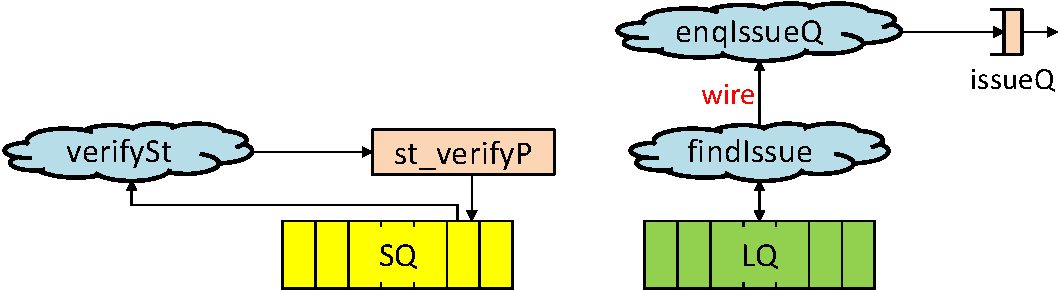
\includegraphics[width=0.7\columnwidth]{fig/lsq_crop.pdf}
    \caption{Internal implementation of LSQ}\label{fig:lsq-impl}
\end{figure}

Figure~\ref{fig:lsq-impl} shows the internal implementation of LSQ.
We use EHRs to store each field of a LQ or SQ entry.
As mentioned earlier, we sequentially verify each SQ entry to ensure that it no longer affect younger loads.
EHR \code{st\_verifyP} points to the SQ entry to be verified next.
Speculative FIFO \code{issueQ} holds loads in LQ that are ready to be issued to execution (i.e., get bypass or access memory).
Method \code{getIssueLd} dequeues this FIFO.
There are three internal rules:
\begin{itemize}
    \item Rule \code{verifySt}: tries to verify that the SQ entry pointed by \code{st\_verifyP} cannot affect younger loads.
    If this is the case, then the rule advances pointer \code{st\_verifyP}, sets field \code{verified} for the SQ entry, and sets field \code{olderStVerified} for applicable LQ entries.
    \item Rule \code{findIssue}: searches LQ for the oldest unissued non-MMIO normal load that is ready to issue.
    The LQ index of the load is recorded in a \emph{wire}.
    \item Rule \code{enqIssue}: reads the value in the wire set by rule \code{findIssue}, and enqueues it into speculative FIFO \code{issueQ}.
\end{itemize}
As we can see, rules \code{findIssue} and \code{enqIssue} should actually be a single rule to ensure atomicity.
However, because \code{issueQ} has the ordering constraint of dequeue before enqueue, the single rule would be ordered after many other rules, and thus, more bypass paths could be introduced.
Since \code{findIssue} performs an associative search, we do not want to introduce bypass paths on it.
Therefore, we split the rule into two, and connect them using a wire.
To make this scheme work, any rule that could affect the LQ entry found by \code{findIssue} must be made conflict with \code{enqIssue}.
Fortunately, only \code{incorrectSpeculation} needs to be conflict with \code{enqIssue}.
It should be noted that since \code{findIssue} does not change any LQ/SQ state, it is fine that \code{enqIssue} fails to fire for whatever reason when \code{findIssue} fires.
However, it is highly desirable to make \code{issueQ} a conflict-free speculative FIFO and put \code{findIssue} and \code{enqIssue} into one rule.

The conflict matrix including the internal rules is (the internal rules are highlighted in red):
\begin{itemize}
    \item \{\code{stqEmpty}, \code{stqFull\_ehrPort0}, \code{ldqFull\_ehrPort0}, \code{noWrongPathLoads}, \code{getOrigBE}, \code{getHit}, \textcolor{red}{\code{findIssue}}\} $<$ \code{deqLd} $<$ \textcolor{red}{\code{verifySt}} $<$ \code{cacheEvict} $<$ \code{updateAddr} $<$ \{\code{getIssueLd}, \code{issueLd}\} $<$ \textcolor{red}{\code{enqIssueQ}} $<$ \{\code{wakeupLdStalledBySB}, \code{deqSt}\} $<$ \code{setAtCommit} $<$ \code{respLd} $<$ \code{updateData} $<$ \{\code{enqLdTag}, \code{enqStTag}\} $<$ \{\code{enqLd}, \code{enqSt}\} $<$ \code{correctSpeculation}
    \item \code{incorrectSpeculation} $<$ \code{correctSpeculation}
    \item \code{incorrectSpeculation} C all others
    \item All others are CF
\end{itemize}
Regarding the problems of \code{issueLd} mentioned before, we have ordered \code{findIssue} before \code{issueLd} and \code{updateAddr}.
That is, the load that calls \code{updateAddr} and \code{issueLd} in the same cycle will not be identified by \code{findIssue}, i.e., no duplicate load issue.

Rules and methods will use the appropriate EHR ports according the conflict matrix.
The only exception is when computing the guard of the \code{enqLd} and \code{enqSt} methods.
The guard is computed using EHR port 0 to avoid bypass from the dequeue methods, and then the computed guard signal is set to a wire checked by the enqueue methods.

\subsubsection{Future Improvement}

\begin{enumerate}
    \item Solve the problem of calling \code{updateAddr} and \code{issueLd} in the same cycle.
    Instead of arbitrating between a newly translated load and a load given by \code{getIssueLd} outside LSQ, we can move this arbitration into LSQ.
    Thus, we always call \code{getIssueLd} outside LSQ to retrieve the load that is ready to issue.
    Then we can hide the problem inside LSQ completely.
    
    \item Merge rules \code{findIssue} and \code{enqIssueQ} into one rule by making \code{issueQ} a conflict-free speculative FIFO.
    
    \item Reconcile fences in case of using a weak memory model is not handled in the optimal way.
    We should put Reconcile fences in LQ and dequeue them earlier than ROB commit time.
\end{enumerate}

\subsubsection{Source Code}
See module \code{mkSplitLSQ} in \code{//procs/lib/SplitLSQ.bsv}.


\subsection{Store Buffer (SB)}\label{sec:sb}

The store buffer (SB) holds committed stores retired from the LSQ.
It can  merge stores for the same cache line and issue multiple requests for different cache lines to the L1 cache.
After a SB entry is issued to the memory system, the entry still stays in SB to merge future stores for the same cache line.
When the L1 cache has retrieved the exclusive permission for the cache line, and L1 cache is updated.
SB is only used in the WMM implementation.

\subsubsection{Interface}

\begin{figure}
\begin{lstlisting}[caption={}]
interface StoreBuffer;
  method Bool isEmpty;
  method Maybe#(SBIndex) getEnqIndex(Addr paddr);
  method Action enq(SBIndex idx, Addr paddr, ByteEn be, Data data);
  method ActionValue#(SBEntry) deq(SBIndex idx);
  method ActionValue#(Tuple2#(SBIndex, SBEntry)) issue;
  method SBSearchRes search(Addr paddr, ByteEn be);
  method Bool noMatchLdQ(Addr paddr, ByteEn be); 
  method Bool noMatchStQ(Addr paddr, ByteEn be); 
endinterface
module mkStoreBufferEhr(StoreBuffer);
  // module implementation
endmodule
\end{lstlisting}
\caption{Interface of SB}\label{fig:sb-ifc}
\end{figure}

Figure~\ref{fig:sb-ifc} shows the interface of SB.
Now we explain each interface method:
\begin{itemize}
    \item Method \code{isEmpty}: returns true if SB is empty.
    This is called typically when a fence instruction is executed for a system instruction is committed.
    
    \item Method \code{getEnqIndex}: returns the index for a SB entry to insert a new store.
    The entry may be a new entry or an existing entry which contains some other stores for the same cache line.
    An \code{Invalid} is returned if no entry can be found.
    
    \item Method \code{enq}: inserts a store into the SB entry at index \code{idx}.
    Argument \code{idx} should be the return value of \code{getEnqIndex}.
    Arguments \code{be} and \code{data} should be shifted to represent a masked 8B aligned data.
    (Lower bits of \code{paddr} are not used.)
    
    \item Method \code{deq}: removes the SB entry at index \code{idx}.
    This is called when L1 gets exclusive permission for the cache line.
    
    \item Method \code{issue}: returns a SB entry that has not been issued to L1 before.
    The entry is not removed from SB.
    L1 will use the address in the SB entry to fetch exclusive permission for the cache line.
    
    \item Method \code{search}: finds bypass and stall for a issuing load in SB.
    Argument \code{be} should be shifted to indicate the valid bytes in a 8B aligned data.
    In case bypass is possible, a 8B aligned data is returned, so the caller needs to shift data before writing to register file.
    
    \item Methods \code{noMatchLdQ} and \code{noMatchStQ}: check if a Lr/Sc/Amo address exists in SB.
    They are called when we try to dequeue a Lr/Sc/Amo from LQ or SQ.
\end{itemize}

\noindent\textbf{Conflict Matrix:}
The conflict matrix of SB is:
\begin{itemize}
    \item \{\code{isEmpty}, \code{issue}, \code{search}\} $<$ \code{deq} $<$ \code{getEnqIndex} $<$ \code{enq}
    \item All others are CF
\end{itemize}

\subsubsection{Implementation}
The implementation uses a vector of EHRs to keep the SB entries.
We use a FIFO \code{freeQ} to keep the indices of free SB entries.
We also use a FIFO \code{issueQ} to keep the indices of SB entries that need to be issued to L1.
A newly allocated entry in method \code{enq} will be inserted into \code{issueQ}, and method \code{issue} will dequeue \code{issueQ} and issue the SB entry pointed by the head of \code{issueQ}.

\subsubsection{Source Code}
See module \code{mkStoreBufferEhr} in \code{//procs/lib/StoreBuffer.bsv}.



\subsection{L1 D Cache}

The L1 D cache takes requests from LSQ and store buffer, and will exchange coherence traffic with L2 cache.

\subsubsection{Interface}

\begin{figure}
\begin{lstlisting}[caption={}]
typedef struct {
  idT id;
  Addr addr;
  Msi toState;
  MemOp op;
  ByteEn byteEn;
  Data data;
  AmoInst amoInst;
} ProcRq#(type idT) deriving(Bits, Eq, FShow);
interface L1ProcReq#(type idT);
  method Action req(ProcRq#(idT) r);
endinterface
interface L1ProcResp#(type idT);
  method Action respLd(idT id, Data resp);
  method Action respLrScAmo(idT id, Data resp);
  method ActionValue#(Tuple2#(LineByteEn, Line)) respSt(idT id);
  method Action evict(LineAddr a);
endinterface
interface DCoCache;
  interface L1ProcReq#(DProcReqId) procReq;
  method Action resetLinkAddr;
  interface Perf#(L1DPerfType) perf;
  interface ChildCacheToParent#(L1Way, void) to_parent;
  interface Get#(L1DCRqStuck) cRqStuck;
  interface Get#(L1DPRqStuck) pRqStuck;
endinterface
module mkDCoCache#(L1ProcResp#(DProcReqId) procResp)(DCoCache);
  // implementation
endmodule
\end{lstlisting}
\caption{Interface of L1 D cache}\label{fig:d-cache-ifc}
\end{figure}

Figure~\ref{fig:d-cache-ifc} shows the interface of D cache.
Struct \code{ProcRq} is the request sent to D cache from the core.
It contains the following fields:
\begin{itemize}
    \item Field \code{id}: is the ID of the request, which is the LQ index or the SB index.
    \item Field \code{addr}: is the physical address of the request.
    \item Field \code{toState}: is the minimum MESI state that is required to process the request for its cache line.
    \item Field \code{op}: is the operation of the request, i.e., load, store, load-reserve, store-conditional, or atomic memory operation (AMO).
    \item Field \code{byteEn}: is valid only for store-conditionals.
    It specifies the bytes to modify in a 8B-aligned data, i.e., \code{byteEn} has been shifted according to the lower bits of the address.
    \item Field \code{data}: is valid only for store-conditionals or AMOs.
    For store-conditionals, it is the 8B-aligned data corresponding to \code{byteEn}, i.e., it has been shifted according to the lower bits of the address..
    For AMOs, it is the data read from the source register, i.e., it is NOT shifted according to address.
    \item Field \code{amoInst}: carries more information about the AMO computation, e.g., fetch-and-add, swap, etc.
\end{itemize}
The \code{DCoCache} interface of the D cache contains the following fields:
\begin{itemize}
    \item Subinterface \code{procReq}: contains a \code{req} method which is called to send new requests to D cache.
    \item Method \code{resetLinkAddr}: clears the reservation made by load-reserves.
    This can be called when the commit stage is processing an exception or interrupt.
    \item Subinterface \code{to\_parent}: contains FIFOs to be connected to the parent L2 cache.
    \item Subinterface \code{perf}: is for querying performance counters in D cache.
    \item Subinterfaces \code{cRqStuck} and \code{pRqStuck}: are for reporting deadlocks for core requests and parent requests, respectively.
\end{itemize}
The \code{L1ProcResp} interface is passed to D cache as an argument.
Its methods will be called when the cache has acquired sufficient MESI state for the cache line to complete the request.
It contains the following fields:
\begin{itemize}
    \item Method \code{respLd}: is to respond a load request with ID \code{id}.
    Argument \code{data} is the 8B-aligned loaded data.
    We still need to shift the data before writing to register file.
    \item Method \code{respLrScAmo}: is to respond a load-reserve or store-conditional or AMO with ID \code{id}.
    In case of a load-reserve, argument \code{data} is the 8B-aligned loaded data, which needs to be shifted before being written back to register file.
    In case of a store-conditional, \code{data} indicates whether the store-conditional succeeds or not (0 means success while 1 means failure).
    In case of an AMO, \code{data} is the original memory value, which can be written back to register file without extra shifting.
    \item Method \code{respSt}: is to respond a store request with ID \code{id}.
    The return value of this method contains the bytes to be modified in the cache line, and the D cache will use this information to update the cache contents.
    \item Method \code{evict}: is called by the D cache when a cache line is evicted (by replacement or invalidation).
    This is needed only in TSO to notify LSQ that some speculative loads may need to be squashed.
\end{itemize}

\noindent\textbf{Conflict Matrix:}
All methods of interface \code{DCocCache} should be conflict free.

\subsubsection{Implementation}

\begin{figure}[t]
    \centering
    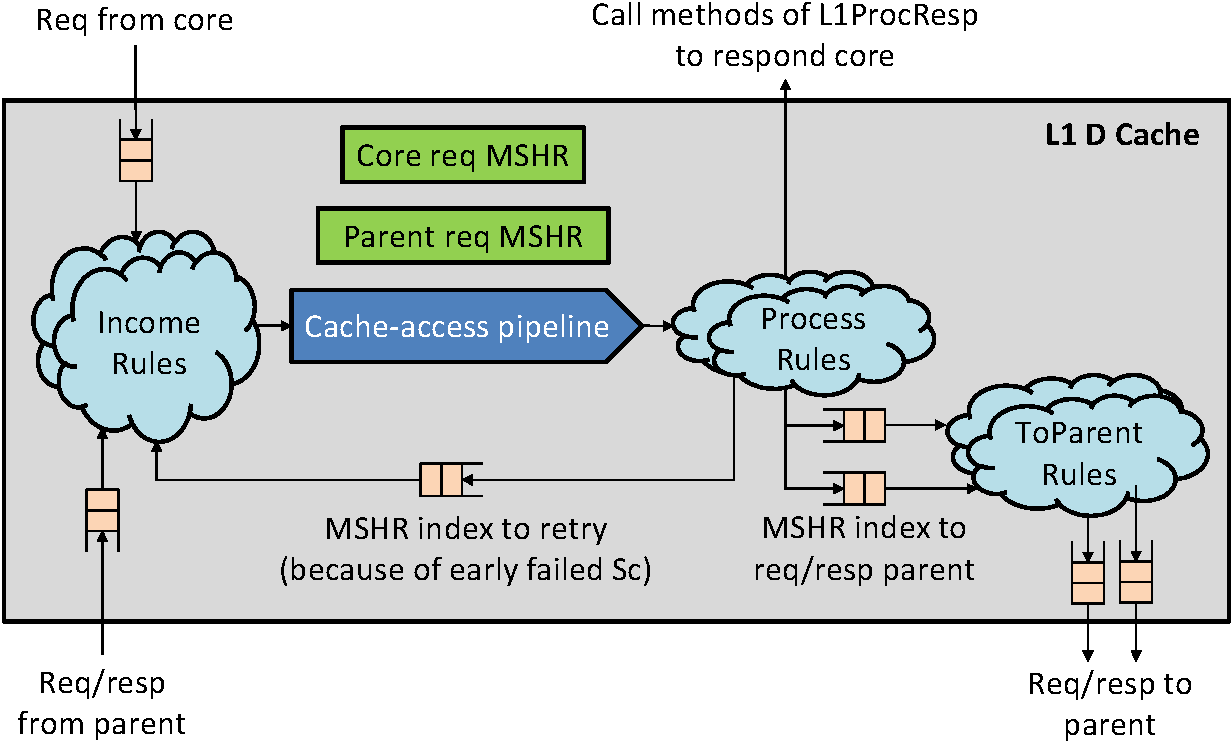
\includegraphics[width=\columnwidth]{fig/d_cache_crop.pdf}
    \caption{Internal implementation of D cache (the names of rules and submodules are different from those in source code)}\label{fig:d-cache-impl}
\end{figure}

Figure~\ref{fig:d-cache-impl} shows the internal implementation of the D cache.
It contains three submodules:
\begin{itemize}
    \item Cache-access pipeline: is a pipeline to access the cache arrays.
    It contains the following three stages:
    \begin{enumerate}
        \item Request tag SRAM.
        \item Get tag SRAM responses, perform tag matching, and request data SRAM.
        \item Get data SRAM responses, and update both data and tag SRAMs.
    \end{enumerate}
    The first and the last stages are interface methods of this submodule, which will be called by the top-level rules of the D cache.
    There are internal bypassing logic in the pipeline to resolve read-after-write hazards.
    \item MSHR for core requests: contains bookkeepings for all the in-flight requests from the core.
    \item MSHR for parent requests: contains bookkeepings for all the in-flight (downgrade) requests from the parent L2 cache.
\end{itemize}

Now we explain how the D cache functions.
Every income message from the core or the parent L2 is entered into the cache-access pipeline by an Income rule.
New requests also need to allocate MSHR entries in these rules.
At the end of the cache-access pipeline, the message is processed by a Process rule.
The Process rule will update states in the MSRH entry and tag/data SRAMs.
In case the rule finds a core request is ready to respond, it will call methods of the \code{L1ProcResp} interface to respond the core.
In case the rule needs to send messages to the parent L2, it will first enter the MSHR index of the request that needs to message L2 into a FIFO, which has the same number of entries as the MSHR and can always be enqueued.
Then the MSHR index will be picked up by a ToParent rule which truly sends a message to L2.

In our coherence protocol, core requests for the same cache line cannot be processed together; they have to be processed one by one.
To ensure this invariant, the core-request MSHR will organize requests for the same cache line as a linked list, and only the head of the list can be truly processed at the Process rule.
When the heading request is responded at the Process rule, it is removed from the MSHR, and the next request in the linked list will be directly swapped into the end of the cache-access pipeline and will be processed by the Process rule.
This increases the throughput if the core keeps requesting on the same cache line.

There is one exception to the above swapping optimization.
If the heading request is a store-conditional and it fails because the cache line is not in the D cache, then we cannot swap the next request into the end of the pipeline.
In this case, we wake up the next request, and let it go through the pipeline.

\subsubsection{Future Improvement}
The current implementation keeps requests for the same cache line in the MSHR.
However, MSHR is a critical resource, and we might want to keep only missing requests in MSHR, instead of those that are idling and waiting for others to complete.

\subsubsection{Source Code}
See the followings:
\begin{itemize}
    \item module \code{mkDCoCache} in \code{//procs/lib/L1CoCache.bsv}, and
    \item module \code{mkL1Bank} in \code{//coherence/src/L1Bank.bsv}.
\end{itemize}


\subsection{L1 I Cache}

The I cache is very similar to the D cache.
The major difference is that I cache sends responses in the same order as the original requests, even though it may processes misses out of order.
The I cache is also coherent with the parent L2.

\subsubsection{Interface}

\begin{figure}
\begin{lstlisting}[caption={}]
interface ICoCache;
  interface Server#(Addr, Vector#(SupSize, Maybe#(Instruction))) to_proc;
  interface ChildCacheToParent#(L1Way, void) to_parent;
  interface Perf#(L1IPerfType) perf;
  interface Get#(L1ICRqStuck) cRqStuck;
  interface Get#(L1IPRqStuck) pRqStuck;
endinterface
module mkICoCache(ICoCache);
  // implementation
endmodule
\end{lstlisting}
\caption{Interface of I cache}\label{fig:i-cache-ifc}
\end{figure}

Figure~\ref{fig:i-cache-ifc} shows the interface of the I cache.
Now we explain the interface:
\begin{itemize}
    \item Subinterface \code{to\_proc}: is a pair of request and response interfaces.
    The request interface takes in an address.
    For this request, the I cache will fetch consecutive instructions starting from this address.
    The fetch will stop until it hits the cache boundary or the number of the fetched instruction reaches the superscalar size.
    The response order is the same as the request order, but the I cache can process multiple misses in parallel.
    \item Other interfaces are similar to those in D cache (Section~\ref{sec:d-cache}).
\end{itemize}

\subsubsection{Implementation}
The implementation is very similar to D cache except that responses are sent to the core in order.

\subsubsection{Source Code}
See the followings:
\begin{itemize}
    \item module \code{mkICoCache} in \code{//procs/lib/L1CoCache.bsv}, and
    \item module \code{mkIBank} in \code{//coherence/src/IBank.bsv}.
\end{itemize}



\subsection{L1 D TLB}\label{sec:d-tlb}
The D TLB contains a fully associative array of page-table entries (PTEs).
A hit takes only one cycle.
The D TLB can process multiple requests and misses in parallel, and will send responses to the core out of order.
Requests in D TLB are speculative, so D TLB also carries speculation masks for the requests.

\subsubsection{Interface}

\begin{figure}
\begin{lstlisting}[caption={}]
typedef struct {
  Addr  addr;
  Bool  write;
} TlbReq deriving(Eq, Bits, FShow);
typedef Tuple2#(Addr, Maybe#(Exception)) TlbResp;
typedef struct {
  instT inst;
  SpecBits specBits;
} DTlbReq#(type instT) deriving(Bits, Eq, FShow);
typedef struct {
  TlbResp resp;
  instT inst;
  SpecBits specBits;
} DTlbResp#(type instT) deriving(Bits, Eq, FShow);
interface DTlb#(type instT);
  method Bool flush_done;
  method Action flush;
  method Action updateVMInfo(VMInfo vm);
  method Bool noPendingReq;
  method Action procReq(DTlbReq#(instT) req);
  method DTlbResp#(instT) procResp;
  method Action deqProcResp;
  interface DTlbToParent toParent;
  interface SpeculationUpdate specUpdate;
  interface Perf#(L1TlbPerfType) perf;
endinterface
module mkDTlb#(function TlbReq getTlbReq(instT inst))(DTlb#(instT));
  // implementation
endmodule
\end{lstlisting}
\caption{Interface of D TLB}\label{fig:d-tlb-ifc}
\end{figure}

Interface \code{DTlb} takes in a type parameter \code{instT}, which is the payload of the instruction that is requesting D TLB.
Argument \code{getTlbReq} for the D TLB module extracts the necessary information from the payload (\code{instT}) to assemble the TLB request (i.e., address and whether it is a write or not).
Now we explain the details of interface \code{DTlb}:
\begin{itemize}
    \item Method \code{flush}: triggers a flush of the TLB.
    \item Method \code{flush\_done}: returns true if the TLB has completed the flush.
    \item Method \code{updateVMInfo}: updates the local copy of some virtual-memory CSRs in the TLB.
    \item Method \code{noPendingReq}: returns true if the TLB does not have any in-flight requests.
    \item Method \code{procReq}: is called by the core to send TLB requests.
    \item Methods \code{procResp} and \code{deqProcResp}: form a FIFO-like dequeue interface.
    \code{procResp} returns a TLB response, and \code{deqProcReq} dequeues it.
    \item Subinterface \code{toParent}: contains FIFO interfaces to be connected to the parent L2 TLB.
    \item Subinterface \code{specUpdate}: manipulates speculative states (Section~\ref{sec:specupdate}).
    \item Subinterface \code{perf}: is for querying performance counters.
\end{itemize}

\noindent\textbf{Conflict Matrix:}
The conflict matrix of the module is:
\begin{itemize}
    \item \code{procResp} $<$ \code{deqProcResp} $<$ \code{procReq} $<$ \code{correctSpeculation}
    \item \code{incorrectSpeculation} C \{\code{deqProcResp}, \code{procReq}\}
    \item \code{toParent} is conflict free with others.
    \item \code{flush}, \code{flush\_done}, \code{noPendingReq}, and \code{updateVMInfo} are implementation dependent.
\end{itemize}

\subsubsection{Implementation}
The implementation has an MSHR which is a vector of EHRs to keep the in-flight requests.
THe MSHR entry will carry the speculation mask for each request.
It also contains a fully associative array containing the cached PTEs.

Method \code{procReq} allocates a MSHR entry for the new request, and searches the fully associative PTE array directly.
If the search hits, then the MSHR entry is marked as ready to respond.
Otherwise, the method marks the request as a miss and requests the parent L2 TLB.
An internal rule \code{doPRs} receives responses from L2 TLB and marks the corresponding requests as ready to respond.
The internal rule \code{doPRs} has the following ordering relations:
\begin{itemize}
    \item \code{deqProcResp} $<$ \code{doPRs} $<$ \code{procReq}
    \item \code{incorrectSpeculation} C \code{doPRs}
\end{itemize}

We implemented an optimization to avoid duplicate requests to L2 TLB.
When we are trying to issue a request to L2 TLB, if another request with the same virtual page number has already issued a request to L2 TLB, then we do not issue a duplicate one.
The \code{doPRs} rule will try to satisfy as many in-flight requests as possible with a single response from L2 TLB.

As for flushing the TLB, after the \code{flush} method is called, the D TLB will stop receiving new requests.
After all in-flight requests have been responded, the fully associative array of PTEs is cleared.
After that, D TLB requests L2 TLB to flush (via the \code{toParent} interface).
The L2 TLB will start flushing after receiving flush requests from both the I TLB and the D TLB, and will respond I and D TLBs when it finishes the flush.
After D TLB receives the flush response from the L2 TLB, the flush is done.

\subsubsection{Future Improvement}
The \code{flush} and \code{flush\_done} methods directly access some flag registers, and create some orderings between methods, which could complicate the scheduling of top-level rules of the processor core.
A better implementation should export the flush functionality as a pair of request and response FIFO interfaces which are conflict-free with each other.

\subsubsection{Source Code}
See module \code{mkDTlb} in \code{//procs/lib/DTlb.bsv}.


\subsection{L1 I TLB}

The L1 I TLB is similar to the D TLB except that it will block in case of a miss (i.e., no hit-under-miss or multiple outstanding misses).
As a consequence, it also sends responses in the order of requests.

\subsubsection{Interface}

\begin{figure}
\begin{lstlisting}[caption={}]
interface ITlb;
  method Bool flush_done;
  method Action flush;
  method Action updateVMInfo(VMInfo vm);
  method Bool noPendingReq;
  interface Server#(Addr, TlbResp) to_proc;
  interface ITlbToParent toParent;
  interface Perf#(L1TlbPerfType) perf;
endinterface
\end{lstlisting}
\caption{Interface of I TLB}\label{fig:i-tlb-ifc}
\end{figure}

Figure~\ref{fig:i-tlb-ifc} shows the interface of the I TLB:
\begin{itemize}
    \item Subinterface \code{to\_proc}: contains a request and response interfaces.
    The request interface takes in a virtual address, and the response interface returns the translation result.
    The response order matches the request order.
    \item Other methods are similar to those in D TLB (Section~\ref{sec:d-tlb})
\end{itemize}

\subsubsection{Implementation}
The implementation uses one register to a missing request, so it will block if there is a miss.
The detailed implementation is a simplified version of the D TLB (Section~\ref{sec:d-tlb}).

\subsubsection{Future Improvement}
We can try to make the I TLB able to support multiple misses.
However, there may not be any improvement because of the locality in instruction fetch.

\subsubsection{Source Code}
See module \code{mkITlb} in \code{//procs/lib/ITlb.bsv}.


\subsection{L2 TLB}
The L2 TLB is still private to the processor core.
It is neither coherent nor inclusive with the L1 I/D TLBs.
It contains a fully associative array for 2MB and 1GB super pages, and a set-associative array for 4KB pages.
The L2 TLB performs hardware page walk in case of a TLB miss.
We support RISC-V Sv39 virtual memory (i.e., 39-bit virtual address), so there are 3 steps in a page walk.
It can support multiple misses and parallel page walks.
It contains a split translation cache to reduce the penalty of page walk.
For each intermediate page-walk step, the split translation cache uses a fully associative array to cache the intermediate page-walk results.
As a result, first few steps in a page can be skipped if we hit in the split translation cache.

\subsubsection{Interface}

\begin{figure}
\begin{lstlisting}[caption={}]
interface L2Tlb;
  method Action updateVMInfo(VMInfo vmI, VMInfo vmD);
  interface L2TlbToChildren toChildren;
  interface TlbMemClient toMem;
  interface Perf#(L2TlbPerfType) perf;
endinterface
module mkL2Tlb(L2Tlb);
  // implementation
endmodule
\end{lstlisting}
\caption{Interface of L2 TLB}\label{fig:l2-tlb-ifc}
\end{figure}

Figure~\ref{fig:l2-tlb-ifc} shows the interface of the L2 TLB:
\begin{itemize}
    \item Method \code{updateVMInfo}: updates the local copy of some virtual-memory CSRs in the TLB.
    \item Subinterface \code{toChildren}: contains FIFO interfaces connected to L1 I/D TLBs.
    \item Subinterface \code{toMem}: contains FIFO interfaces connected to the coherent memory system (or more precisely, the shared L2 cache).
    \item Subinterface \code{perf}: is for querying the performance counters in the TLB.
\end{itemize}

\noindent\textbf{Conflict Matrix:}
Most methods should be conflict free.

\subsubsection{Implementation}

\begin{figure}
    \centering
    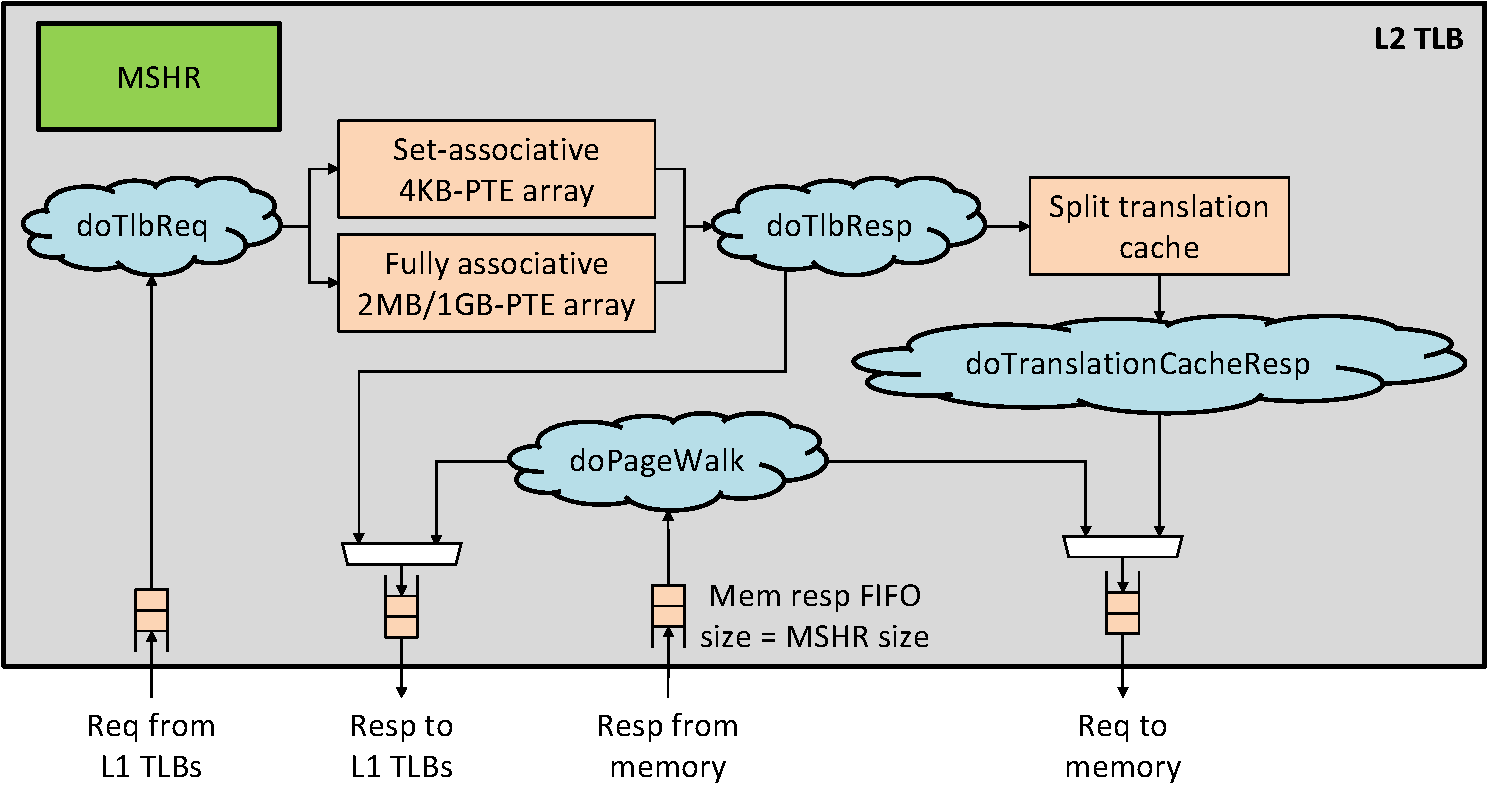
\includegraphics[width=\columnwidth]{fig/l2_tlb_crop.pdf}
    \caption{Internal implementation of L2 TLB}\label{fig:l2-tlb-impl}
\end{figure}

Figure~\ref{fig:l2-tlb-impl} shows the internal implementation of L2 TLB.
All the in-flight requests from L1 TLBs are kept in the MSHR, which is a vector of EHRs.

Every new request from the L1 TLBs is first processed by the \code{doTlbReq} rule, which allocates a new MSHR entry for the request and starts accessing the leaf-PTE arrays, i.e., both the set-associative arrays for 4KB PTEs and the fully associative array for 2MB/1GB PTEs.
Rule \code{doTlbResp} gets the response from the leaf-PTE arrays.
If we hit in the arrays, then we can directly respond the L1 TLB.
Otherwise, we continue to request the split translation cache to prepare for page walk.
Rule \code{doTranslationCacheResp} gets the response from the split translation cache, decides which steps of the page walk can be skipped, and starts the page walk by requesting the memory system.
Rule \code{doPageWalk} gets the response from the memory system, i.e., the result of the previous page walk step.
If there is a page fault or we have reached the leaf PTE, then we can respond L1 TLB.
Otherwise, we continue the page walk by requesting the memory system again.
This rule also refills the leaf-PTE arrays and the split translation cache.

We implemented an optimization to avoid duplicate requests to memory.
When we are trying to issue a request to memory for page walking, if another request has already issued the same memory request, then we do not issue a duplicate one.
The \code{doPageWalk} rule will try to satisfy as many in-flight requests as possible with a single response from memory.

\subsubsection{Source Code}
See module \code{mkL2Tlb} in \code{//procs/lib/L2Tlb.bsv}.


\subsection{FPU}~\label{sec:fpu}

The FPU module contains the following floating-point execution units:
\begin{itemize}
    \item Simple unit: performs simple operations, e.g., converting between integer and floating point.
    \item FMA (fused-multiply-add) unit: performs add, multiply and FMA.
    \item Divide unit: performs division.
    \item Square-root unit: calculates the square root.
\end{itemize}
Every floating point instruction will use one of the execution units.
Since different execution units can have different latency and throughput, FPU will respond out of order.
FPU also keeps the speculation mask for each instruction inside, so wrong-path instructions will be dropped inside FPU and will not be outputted.

\subsubsection{Interface}

\begin{figure}
\begin{lstlisting}[caption={}]
interface FpuExec;
  method Action exec(FpuInst fpu_inst, Data rVal1, Data rVal2, Data rVal3,
  Maybe#(PhyDst) dst, InstTag tag, SpecBits specBits);
  method ActionValue#(FpuResp) simpleResp;
  method ActionValue#(FpuResp) fmaResp;
  method ActionValue#(FpuResp) divResp;
  method ActionValue#(FpuResp) sqrtResp;
  interface SpeculationUpdate specUpdate;
endinterface
module mkFpuExecPipeline(FpuExec);
  // implementation
endmodule
\end{lstlisting}
\caption{Interface of FPU}\label{fig:fpu-ifc}
\end{figure}

Figure~\ref{fig:fpu-ifc} shows the interface of FPU:
\begin{itemize}
    \item Method \code{exec}: is called to send a new floating point instruction \code{fpu\_inst} into the FPU.
    This method will dispatch the instruction to the appropriate execution unit.
    Notice that argument \code{specBits} is used to kill wrong-path instructions inside FPU.
    \item Methods \code{simpleResp}, \code{fmaResp}, \code{divResp}, \code{sqrtResp}: return the responses from the simple, FMA, divide, and square-root units, respectively.
    Wrong-path instructions will not be returned.
    \item Subinterface \code{specUpdate}: manipulates speculative states (Section~\ref{sec:specupdate}).
\end{itemize}

\noindent\textbf{Conflict Matrix:}
\begin{itemize}
    \item \{\code{simpleResp}, \code{fmaResp}, \code{divResp}, \code{sqrtResp}\} $<$ \code{exec}.
    \item \code{simpleResp}, \code{fmaResp}, \code{divResp}, \code{sqrtResp} are conflict-free with each other.
\end{itemize}


\subsubsection{Implementation}
The simple unit is just a speculation FIFO (Section~\ref{sec:specfifo}).
For an instruction that goes into the simple unit, the \code{exec} method directly computes the result and enters the result into the FIFO.

The FMA, divide and square-root units are implemented in the same way.
For each unit, the real computation pipeline is a Xilinx IP core.
There is a speculative poisoned FIFO (Section~\ref{sec:specpoisonfifo}) accompanying the pipeline.
The FIFO contains all the in-flight instructions in the pipeline.
When mis-speculation happens, wrong-path instructions will be poisoned in the FIFO.
And when the wrong-path instruction is dequeued from the pipeline and the FIFO, it will be dropped.

\subsubsection{Source Code}
See the followings:
\begin{itemize}
    \item module \code{mkFpuExecPipeline} in \code{//procs/lib/Fpu.bsv}, and
    \item all modules in \code{//fpgautils/lib/XilinxFpu.bsv}.
\end{itemize}


\subsection{Integer Multiplier and Divider}

This module is very similar to the FPU (Section~\ref{sec:fpu}).
The only difference is that this module contains an integer-multiply unit and an integer-divide unit instead of four floating-point execution units.
We will skip the details of this module.

\subsubsection{Source Code}
See the followings:
\begin{itemize}
    \item module \code{mkMulDivExec} in \code{//procs/lib/MulDiv.bsv},
    \item module \code{mkXilinxIntMul} in \code{//fpgautils/lib/XilinxIntMul.bsv}, and
    \item module \code{mkXilinxIntDiv} in \code{//fpgautils/lib/XilinxIntDiv.bsv}.
\end{itemize}


\subsection{CSR Register File}
The CSR register file contains all the CSRs.
Besides the official CSRs in the RISC-V ISA, it also includes two custom CSRs:
\begin{itemize}
    \item The stats CSR: controls whether performance counters will be incremented or not.
    When the stats CSR of one processor core is written, the write will be automatically propagated to all other cores.
    \item The terminate CSR: will terminate the whole processor when any value is written to it.
\end{itemize}

\subsubsection{Interface}

\begin{figure}
\begin{lstlisting}[caption={}]
interface CsrFile;
  method Data rd(CSR csr);
  method Action csrInstWr(CSR csr, Data x);
  method Bool fpuInstNeedWr(Bit#(5) fflags, Bool fpu_dirty);
  method Action fpuInstWr(Bit#(5) fflags);
  method Maybe#(Interrupt) pending_interrupt;
  method ActionValue#(Addr) trap(Trap t, Addr pc, Addr faultAddr);
  method ActionValue#(Addr) sret;
  method ActionValue#(Addr) mret;
  method VMInfo vmI;
  method VMInfo vmD;
  method CsrDecodeInfo decodeInfo;
  method Action incInstret(SupCnt x);
  method Action setTime(Data t);
  method Bit#(1) getMSIP;
  method Action setMSIP(Bit#(1) v);
  method Action setMTIP(Bit#(1) v);
  method Bool doPerfStats;
  method ActionValue#(Bool) sendDoStats;
  method Action recvDoStats(Bool s);
  method ActionValue#(void) terminate;
endinterface
module mkCsrFile#(Data hartid)(CsrFile);
  // implementation
endmodule
\end{lstlisting}
\caption{Interface of CSR register file}\label{fig:csr-file-ifc}
\end{figure}

Figure~\ref{fig:csr-file-ifc} shows the interface of the CSR register file:
\begin{itemize}
    \item Method \code{rd}: returns the value of a given CSR.
    \item Method \code{csrInstWr}: updates a CSR when a \inst{CSRRW} instruction is committed.
    \item Method \code{fpuInstNeedWr}: returns whether a floating-point instruction needs to update the \code{fcsr} CSR.
    \item Method \code{fpuInstWr}: updates the \code{fcsr} CSR when a a floating-point instruction is committed.
    \item Method \code{pending\_interrupt}: returns any pending interrupts.
    \item Method \code{trap}: updates the CSRs for an exception or interrupt (at commit stage), and returns the next PC (i.e., the entry to the interrupt/exception handler).
    \item Methods \code{sret} and \code{mret}: udpates the CSRs when a return-from-trap instruction (\inst{SRET} or \inst{MRET}) is committed, and returns the next PC.
    \item Methods \code{vmI}, \code{vmD} and \code{decodeInfo}: return some CSR contents that may be used in other parts of the processor.
    \item Method \code{incInstret}: increments the \code{minstret} CSR by the number of committed instructions in this cycle.
    \item Method \code{setTime}: updates the local copy of the machine time (the original machine time register is maintained in the uncore).
    \item Methods \code{getMSIP}, \code{setMSIP}, \code{setMTIP}: provide accesses on the interrupt pending bits (such accesses are made by the uncore).
    \item Method \code{doPerfStats}: returns whether performance counters should be incremented or not.
    \item Methods \code{sendDoStats} and \code{recvDoStats}: propagate the changes on the stats CSR between processor cores.
    \item Method \code{terminate}: indicates the whole processor should be shutdown because of writes on the terminate CSR, if the method is ready.
\end{itemize}
The module argument \code{hartid} is the core ID.

\subsubsection{Implementation}
Since there is no read-after-write hazards on CSRs, we use Bluespec \code{mkConfigReg} to implement each CSR.
This avoids unncessary constraints on rule scheduling.

\subsubsection{Source Code}
See module \code{mkCsrFile} in \code{//procs/lib/CsrFile.bsv}.


\subsection{MMIO Hanlder}\label{sec:mmio-core}

The MMIO handler delivers the following MMIO accesses made inside the processor core to the uncore platform:
\begin{itemize}
    \item boot-rom accesses to fetch instructions, and
    \item MMIO data accesses made by memory instructions in LSQ.
\end{itemize}
The module also processes the following requests from the uncore platform:
\begin{itemize}
    \item posting timer interrupt (the \code{MTIP} bit),
    \item reading and writing the software interrupt bit (\code{MSIP}), and
    \item updating the copy of the machine time in CSR register file.
\end{itemize}

\subsubsection{Interface}

\begin{figure}
\begin{lstlisting}[caption={}]
interface MMIOCoreToPlatform;
  interface FifoDeq#(MMIOCRq) cRq;
  interface FifoEnq#(MMIOPRs) pRs;
  interface FifoEnq#(MMIOPRq) pRq;
  interface FifoDeq#(MMIOCRs) cRs;
  method Action setTime(Data t);
endinterface
interface MMIOCore;
  method Bool isMMIOAddr(Addr addr);
  method Action dataReq(MMIOCRq r);
  method MMIODataPRs dataRespVal;
  method Action dataRespDeq;
  method Action setHtifAddrs(Addr toHost, Addr fromHost);
  method Bool hasPendingPRq;
  interface MMIOCoreToPlatform toP;
endinterface
interface MMIOInstToCore;
  interface FifoDeq#(Tuple2#(Addr, SupWaySel)) instReq;
  interface FifoEnq#(Vector#(SupSize, Maybe#(Instruction))) instResp;
  method Action setHtifAddrs(Addr toHost, Addr fromHost);
endinterface
interface MMIOCoreInput;
  interface MMIOInstToCore fetch;
  method Bit#(1) getMSIP;
  method Action setMSIP(Bit#(1) v);
  method Action setMTIP(Bit#(1) v);
  method Action setTime(Data t);
  method Bool noInflightCSRInstOrInterrupt;
endinterface
module mkMMIOCore#(MMIOCoreInput inIfc)(MMIOCore);
  // implementation
endmodule
\end{lstlisting}
\caption{Interface of MMIO handler}\label{fig:mmio-core-ifc}
\end{figure}

Figure~\ref{fig:mmio-core-ifc} shows the interface of the MMIO handler module.
Module interface \code{MMIOCore} contains the following fields:
\begin{itemize}
    \item Method \code{isMMIOAddr}: returns true if physical address \code{addr} is a MMIO address.
    The \code{tohost} and \code{fromhost} addresses used in the BBL (Berkeley boot loader) are also considered as MMIO addresses.
    \item Method \code{dataReq}: sends a MMIO requests to uncore platform.
    \item Methods \code{dataRespVal} and \code{dataRespDeq}: gets the MMIO response from uncore platform.
    \item Method \code{setHtifAddrs}: tells the MMIO handler what are the \code{tohost} and \code{fromhost} addresses.
    \item Method \code{hasPendingPRq}: returns true if the handler has received a request from the uncore platform.
    The rename stage calls this method to stop renaming and let the MMIO handler to complete the request from uncore platform.
    This can avoid conflicting accesses on CSRs, because rename stage checks interrupts while the uncore-platform request may post interrupts.
    \item Subinterface \code{toP}: contains FIFO interfaces connected to the uncore platform.
    It also contains a \code{setTime} methods to let the uncore platform to update the copy of machine time in CSR register file.
\end{itemize}
Interface \code{MMIOCoreInput} is the argument passed  to the module.
It contains the following fields:
\begin{itemize}
    \item Subinterface \code{fetch}: contains FIFO interfaces of the fetch pipeline to access boot rom in the uncore platform.
    \item Methods \code{getMSIP}, \code{setMSIP}, \code{setMTIP}, and \code{setTime}: are from CSR register file to update the CSRs.
    \item Method \code{noInflightCSRInstOrInterrupt}: returns true if the ROB  does not contain any \inst{CSRRW} instructions or interrupt instructions.
    The MMIO handler processes a request from uncore platform only when this method returns true to avoid conflicting accesses on CSRs.
    (Exceptions do not touch the interrupt bits, so it is ok for ROB to contain instructions with exceptions.)
    This may be over conservative, because RISC-V ISA seems to guarantee that software cannot modify \code{MSIP} and \code{MTIP} bits.
\end{itemize}

\subsubsection{Implementation}
The module allows only one outstanding a MMIO request from the core, because MMIO accesses are believed to be rare.

When the module receives a request from the uncore platform to read or write the interrupt pending bits, it takes actions only when the \code{noInflightCSRInstOrInterrupt} method of the module argument interface returns true.
After taking the action, it sends a response to the uncore platform.

\subsubsection{Future Improvement}
As mentioned earlier, checking method \code{noInflightCSRInstOrInterrupt} before handling requests from uncore platform may be too conservative.
We should consider removing this check in the future.

\subsubsection{Source Code}
See module \code{mkMMIOCore} in \code{//procs/lib/MMIOCore.bsv}.


\subsection{Fetch Pipeline}

The fetch pipeline performs address-translation of PC, superscalar instruction-fetch and decode, and various branch predictions.
It contains the I cache, I TLB, PC register, branch predictors, and decode logic.

\subsubsection{Interface}

\begin{figure}
\begin{lstlisting}[caption={}]
interface MMIOInstToCore;
  interface FifoDeq#(Tuple2#(Addr, SupWaySel)) instReq;
  interface FifoEnq#(Vector#(SupSize, Maybe#(Instruction))) instResp;
  method Action setHtifAddrs(Addr toHost, Addr fromHost);
endinterface
interface FetchStage;
  interface Vector#(SupSize, SupFifoDeq#(FromFetchStage)) pipelines;
  interface ITlb iTlbIfc;
  interface ICoCache iMemIfc;
  interface MMIOInstToCore mmioIfc;
  method Action start(Addr pc);
  method Action setWaitRedirect;
  method Action redirect(Addr pc);
  method Action done_flushing();
  method Action train_predictors(Addr pc, Addr next_pc, IType iType, Bool taken, DirPredTrainInfo dpTrain, Bool mispred);
  interface Perf#(DecStagePerfType) perf;
endinterface
module mkFetchStage(FetchStage);
  // implementation
endmodule
\end{lstlisting}
\caption{Interface of fetch pipeline}\label{fig:fetch-fic}
\end{figure}

Figure~\ref{fig:fetch-fic} shows the interface of the fetch pipeline:
\begin{itemize}
    \item Subinterface \code{pipelines}: is a vector of FIFO-dequeue interfaces.
    The rename stage will dequeue these FIFO interfaces to retrieve decoded instructions.
    The rename stage should always first dequeue FIFO 0, then FIFO 1, and so on.
    \item Subinterface \code{iTlbIfc}: returns the interface of the I TLB.
    We will connect it to the L2 TLB, and the commit stage may call the flush method of it.
    \item SubInterface \code{iMemIfc}: returns the interface of the I cache.
    We will connect it to the L2 cache in the uncore.
    \item Subinterface \code{mmioIfc}: contains FIFO interfaces to fetch instructions from the boot rom in the uncore.
    This interface will be passed to the MMIO handler module (Section~\ref{sec:mmio-core}).
    \item Method \code{start}: starts the fetch pipeline to fetch instructions.
    This is called when the processor starts.
    \item Method \code{setWaitRedirect}: is called when the back-end of the processor decides to redirect the PC, but still does not know the next PC.
    This method stops instruction fetch (instructions already in the fetch pipeline will still flow through and get killed at rename stage as wrong-path instructions) and starts waiting for the method call of \code{redirect}.
    This method helps reduce the unnecessary fetch of wrong-path instructions.
    \item Method \code{redirect}: changes the PC register, and increments the local copy of the epoch.
    The original epoch is in the epoch manager (Section~\ref{sec:epoch}).
    It should be noted that instruction fetch will not be resumed, because we conservatively anticipate that the back-end may still have things to flush.
    Instruction fetch will be resumed when method \code{done\_flushing} is called.
    \item Method \code{done\_flushing}: resumes instruction fetch.
    \item Method \code{train\_predictors}: trains the branch predictors.
    \item Subinterface \code{perf}: is for querying performance counters.
\end{itemize}

\subsubsection{Implementation}

\begin{figure}
    \centering
    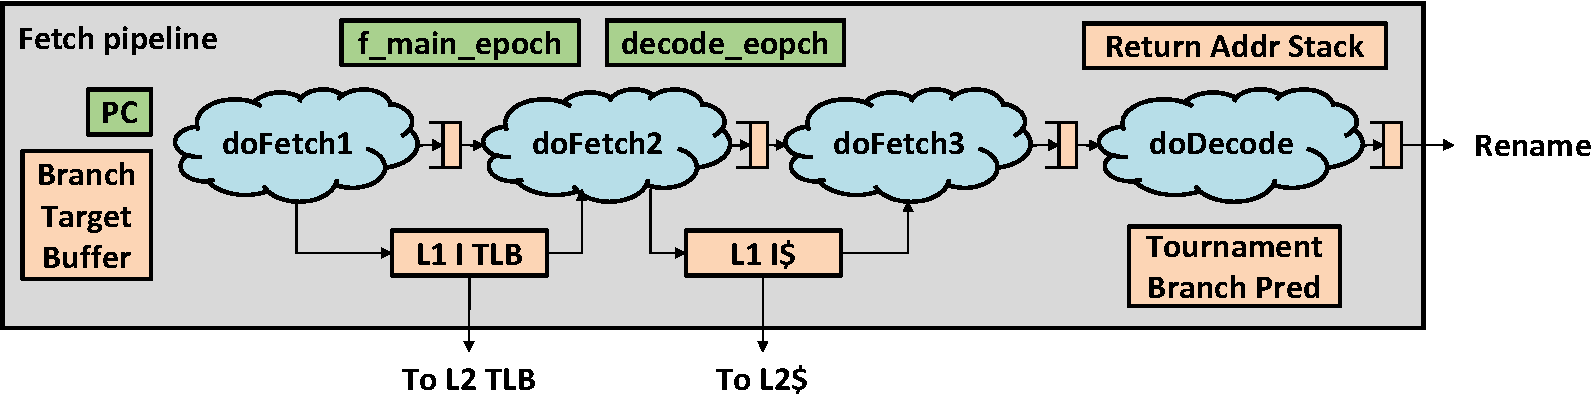
\includegraphics[width=\columnwidth]{fig/fetch_crop.pdf}
    \caption{Implementation of fetch pipeline}\label{fig:fetch-impl}
\end{figure}

Figure~\ref{fig:fetch-impl} shows the internal implementation of the fetch pipeline.
There are three internal rules:
\begin{itemize}
    \item Rule \code{doFetch1}: initiates the address translation of PC, and use BTB to update the PC.
    \item Rule \code{doFetch2}: retrieves the translated physical address and starts accessing I cache (or boot rom via the \code{mmioIfc} interface) to fetch instructions.
    \item Rule \code{doFetch3}: cuts the fetched data into a vector of instructions (because we are doing superscalar fetch).
    \item Rule \code{doDecode}: performs branch predictions and decodes instructions.
\end{itemize}
To ensure the correctness of branch redictions, the fetch pipeline contains two epochs:
\begin{itemize}
    \item EHR \code{f\_main\_epoch}: is the copy of the epoch in the epoch manager (Section~\ref{sec:epoch}), and is incremented by the \code{redirect} method.
    \item EHR \code{decode\_epoch}: is local to the fetch pipeline, and is incremented when the \code{doDecode} rule redirects PC according to branch predictors.
\end{itemize}
Rule \code{doFetch1} tag the request to I TLB with both epochs, and both epochs will flow through the pipeline with the fetched instructions.
Rule \code{doDecode} checks both epochs to drop wrong-path instructions, and only \code{f\_main\_epoch} is outputted to the rename stage with the correct-path instruction.

\subsubsection{Source Code}
See module \code{mkFetchStage} in \code{//procs/RV64G\_OOO/FetchStage.bsv}.



\subsection{Rename Stage}

The rename stage is logically a single rule that retrieves instructions from the fetch pipeline, performs superscalar renaming, and enters the instructions to the reservation stations of the execution pipelines.
In implementation, this stage is implemented using the following mutually exclusive rules:
\begin{itemize}
    \item Rule \code{doRenaming\_wrongPath}: drops wrong-path instructions.
    This rule can drop multiple wrong-path instructions in a cycle.
    \item Rule \code{doRenaming\_Trap}: processes a single instruction with exception or a single interrupt.
    As mentioned earlier, this rule can fire only if the ROB is empty, and this rule will call method \code{setWaitRedirect} of the fetch pipeline and increment the epoch in the epoch manager.
    \item Rule \code{doRenaming\_SystemInst}: processes a single system instruction.
    As mentioned earlier, this rule can fire only if the ROB is empty, and this rule will call method \code{setWaitRedirect} of the fetch pipeline and increment the epoch in the epoch manager.
    \item Rule \code{doRenaming}: processes normal instructions without exceptions.
    This rule can rename multiple instructions in a cycle until one of the followings happens:
    \begin{itemize}
        \item We have reached the limit of superscalarity.
        \item We see a wrong-path instruction or instruction with exception.
        \item There is not enough hardware resource to process the instruction (e.g., not enough space in the reservation station, or not enough enqueue port to LSQ).
    \end{itemize}
    If one instruction can be dispatched to multiple execution pipelines (e.g., an ALU instruction), we try to send it to the pipeline whose reservation station has more free entries.
\end{itemize}
All the above renaming rules are stalled if there is a pending request from the uncore to read or write interrupt bits (Section~\ref{sec:mmio-core}).

\subsubsection{Source Code}
See module \code{mkRenameStage} in \code{//procs/RV64G\_OOO/RenameStage.bsv}.


\subsection{ALU Execution Pipeline}

The ALU execution pipeline executes ALU and branch instructions (including \inst{CSRRW} instructions).
To sustain peak throughput for ALU instructions with back-to-back dependencies, the pipeline contains bypass logic and wakes up dependent instructions aggressively.

\subsubsection{Interface}

\begin{figure}
\begin{lstlisting}[caption={}]
interface AluExeInput;
  method RegsReady sbCons_lazyLookup(PhyRegs r);
  method Data rf_rd1(PhyRIndx rindx);
  method Data rf_rd2(PhyRIndx rindx);
  method Data csrf_rd(CSR csr);
  method Addr rob_getPC(InstTag t);
  method Addr rob_getPredPC(InstTag t);
  method Action rob_setExecuted(InstTag t, Maybe#(Data) csrData, ControlFlow cf);
  method Action fetch_train_predictors(FetchTrainBP train);
  method Action setRegReadyAggr(PhyRIndx dst);
  interface Vector#(2, SendBypass) sendBypass;
  method Action writeRegFile(PhyRIndx dst, Data data);
  method Action redirect(Addr new_pc, SpecTag spec_tag, InstTag inst_tag);
  method Action correctSpec(SpecTag t);
  method Bool doStats;
endinterface
interface AluExePipeline;
  interface Vector#(TMul#(2, AluExeNum), RecvBypass) recvBypass;
  interface ReservationStationAlu rsAluIfc;
  interface SpeculationUpdate specUpdate;
  method Data getPerf(ExeStagePerfType t);
endinterface
module mkAluExePipeline#(AluExeInput inIfc)(AluExePipeline);
  // implementation
endmodule
\end{lstlisting}
\caption{Interface of ALU execution pipeline}\label{fig:alu-exe-pipe-ifc}
\end{figure}

Figure~\ref{fig:alu-exe-pipe-ifc} shows the interface of the ALU execution pipeline.
Interface \code{AluExeInput} is the input argument to the module.
It contains the following fields:
\begin{itemize}
    \item Methods \code{sbCons\_lazyLookup}, \code{rf\_rd1} and \code{rf\_rd2}: read the conservative scoreboard and physical register file.
    \item Method \code{csrf\_rf}: reads the CSR register file.
    This is called by the module in case of the \inst{CSRRW} instruction.
    \item Methods \code{rob\_getPC} and \code{rob\_getPredPC}: retrieve PC and predicted PC (by the fetch pipeline), respectively, from the corresponding ROB entry.
    \item Method \code{rob\_setExecuted}: sets the ROB entry as executed, so the instruction can be committed if it is the oldest in ROB.
    \item Method \code{fetch\_train\_predictors}: trains the branch predictors in the fetch pipeline.
    \item Method \code{setRegReadyAggr}: wakes up dependent instructions in all the reservation stations, and sets the aggressive scoreboard.
    \item Subinterface \code{sendBypass}: is called by the module to send out data forwardings to other execution pipelines and itself.
    \item Method \code{writeRegFile}: writes the physical register file.
    \item Method \code{redirect}: redirects the fetch pipeline, increments the epoch in the epoch manager, and calls the global speculation updater to kill wrong-path instructions (i.e., call the \code{incorrectSpeculation} method of every module).
    This method is called by the ALU execution pipeline in case of branch mispreditions.
    \item Method \code{correctSpec}: calls the global speculation updater to release a speculation tag (i.e., call the \code{correctSpeculation} method of every module).
    This method is called by the ALU execution pipeline in case of correct branch preditions.
    \item Method \code{doStats}: returns whether performance counters should be incremented or not.
\end{itemize}
The module interface \code{AluExePipeline} contains the following fields:
\begin{itemize}
    \item Subinterface \code{recvBypass}: receives the data forwardings sent by other execution pipelines and itself.
    That is, interface \code{sendBypass} in the module argument will call this interface.
    \item Subinterface \code{rsAluIfc}: returns the reservation station inside the pipeline.
    \item Subinterface \code{specUpdate}: manipulates speculative states (Section~\ref{sec:specupdate}).
    \item Method \code{getPerf}: is for querying performance counters.
\end{itemize}

\subsubsection{Implementation}

\subsection{FPU (and Integer Multiply/Divide) Execution Pipeline}

The FPU execution pipeline is very similar to the ALU execution pipeline (Section~\ref{sec:alu-exe-pip}).
The only difference is that instead of computing the result in a single rule, the \code{doExe} rule sends the instruction to the FPU module or the integer multiply and divide module for computation.
The \code{doFinish} rule will pick up the instructions outputted by these two submodules.
We skip the details here.

\subsubsection{Source Code}
See module \code{mkFpuMulDivExePipeline} in \code{//procs/RV64G\_OOO/FpuMulDivExePipeline.bsv}.


\section{Uncore}

\end{document}
